% !TEX root = ../Rulebook.tex

In this chapter the general rules will be explained that are valid for all tests. This chapter is seperated into the sections robot, arena environment, Service Areas and Objects.

%Each of the particular tests defined later in this document may define its own scenario. In this document, a scenario consists of elements such as the
%
%\begin{itemize}
%	\item environment,
%	\item Objects that affect navigation,
%	\item Objects that are to be manipulated,
%	\item Objects with which robots interact,
%	\item number of robots allowed per team,
%	\item number of teams competing simultaneously in the same arena,
%	\item task to be performed by a team, and
%	\item the criteria for evaluating a team's performance.
%\end{itemize}
%
%In order to avoid excessive development efforts for each specific test and to allow reuse of partial functionalities the scenarios are built from a reasonably small set of components, which are later put together in different ways. This section describes these elements.

\section{Robots}
The robots used for competition shall satisfy professional quality standards. The concrete definition of these standards is to be assessed by the TC, comprising aspects such as sturdy construction, general safety, and robust operation. It is not required that the robots are certified for industrial use.

\subsection{Design and Constraints} \label{ssec:RobotDesignAndConstraints}
%The robots need to comply with certain size constraints. A robot, including all parts attached to it as used in the competition, must be able to move by itself into a configuration so that it fits into a box of side lengths 80 cm x 55 cm x 110 cm (length x width x height). If all the robot's parts, such as manipulator or anything able to protrude outside of the previously specified box, are fully extended, the system must still not exceed a box of side lengths 120 cm x 80 cm x 160 cm (length x width x height). The organizers may specify further constraints, such as weight limits. If a team would like to apply a robot with deviating robot dimensions, it should contact the TC. Exceptions for specific robots are possible in case of small differences.


There are no constraints regarding the size and weight of the used robots, but that they have to fit in the arena defined in section \ref{sec:ArenaDesign}. The minimum passage width is $80\si{\centi\meter}$. The used robots must be able to maneuver in that space.\par

The used batteries may not exceed 500Wh of capacity for safety. 300Wh of capacity is recommended. The maximum voltage that is allowed on the robotic system is 60 V DC.

See subsection \ref{ssec:RobotBehaviorAndSafety} as well.\par 

The maximum speed of the robots may not exceed 1.5 m/s. The robot should also be able to stop within a reasonable distance on concrete floor.

\par
Electric, pneumatic, and hydraulic actuation mechanisms are permitted, provided that they are constructed and produced according to professional standards and meet safety constraints. Combustion engines and any kind of explosives are strictly forbidden. Robots may not pollute or harm their environment in any way, e.g. by loss of chemicals or oil, spilling liquids, or exhausting gases.
\par
Further, the following assumptions are made about the kind of robots used in the competition:
\par
\begin{itemize}
	\item At least one of the robots used by a team is mobile and moves on wheels. No specific assumptions are made about the kinematic design, but the mobile robots should be able to move on basically flat, sufficiently firm surfaces. Aerial robots are not allowed in this competition. 
	\item The robots have at least one manipulator and are able to grasp Objects, which are used in the individual task. See Table~\ref{tab:manipulation_objects}, Table~\ref{tab:manipulation_objects_rockin} and Table~\ref{tab:new_objects1} as well as Table~\ref{tab:new_objects2}.
	\item The manipulator of the robot should be designed and mounted on the robot such that it can grasp Objects from different heights between $0\si{\centi\meter}$ and $40\si{\centi\meter}$ above the floor.
	\item The robots use sensors to obtain information about their whereabouts in the environment and the task-relevant Objects. The major types of sensors that may be used by the robots include:
	\begin{itemize}
		\item Laser range finders (cf. models by Hokuyo or Sick)
		\item Color CCD cameras (cf. any kind of USB camera)
		\item 3D cameras (cf. any kind of camera with depth information)
	\end{itemize}
	\item The design of the scenario should be such that the robots can solve the tasks safely and robustly using (all or a subset of) these sensors.
\end{itemize}
If there are even vague doubts about the eligibility of using particular designs, parts, or mechanisms, the team should consult the TC well in advance.
The TC may require that robots are equipped with a wireless communication device of some sort (e.g. 802.11n), in order to communicate task specifications to the robots. Figure~\ref{fig:example_robots} shows three examples how a robot suitable to the competition can look like. 
\begin{figure} [h!]
	\begin{center}
		\subfloat{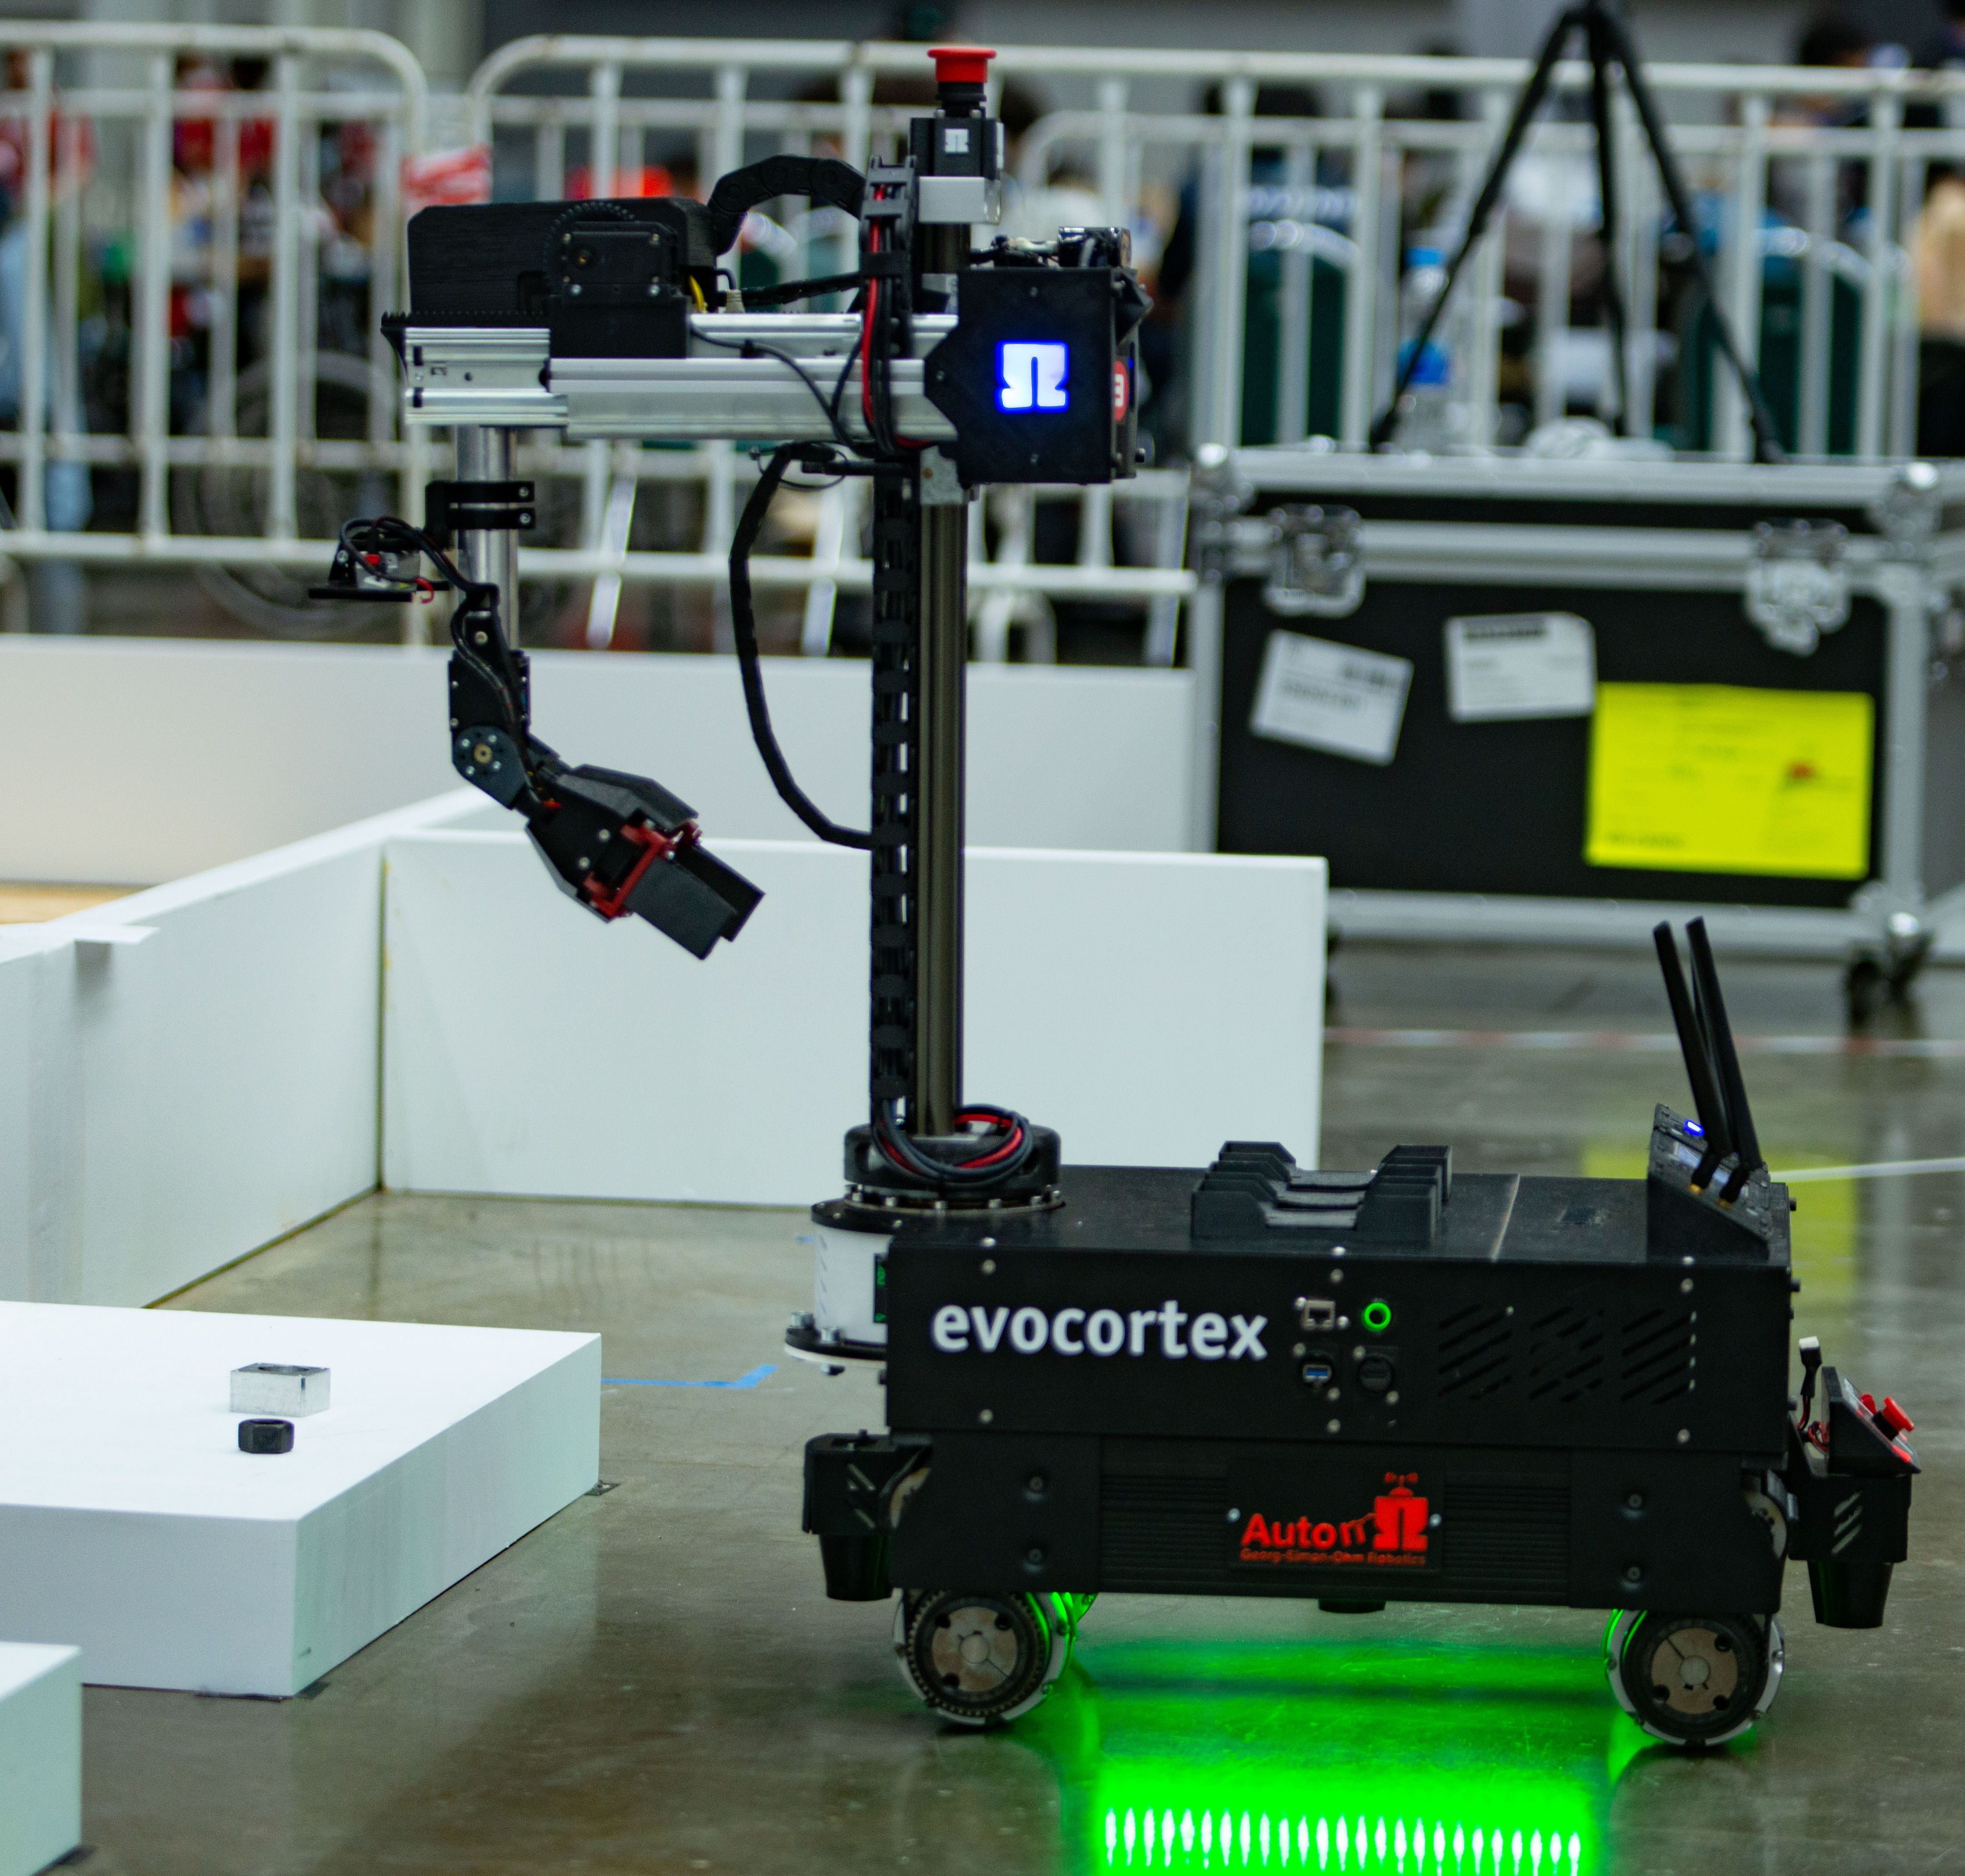
\includegraphics[width=0.3\textwidth]{./images/robots/AutonOhm_Ohmn3.jpg}} \hfill
		\subfloat{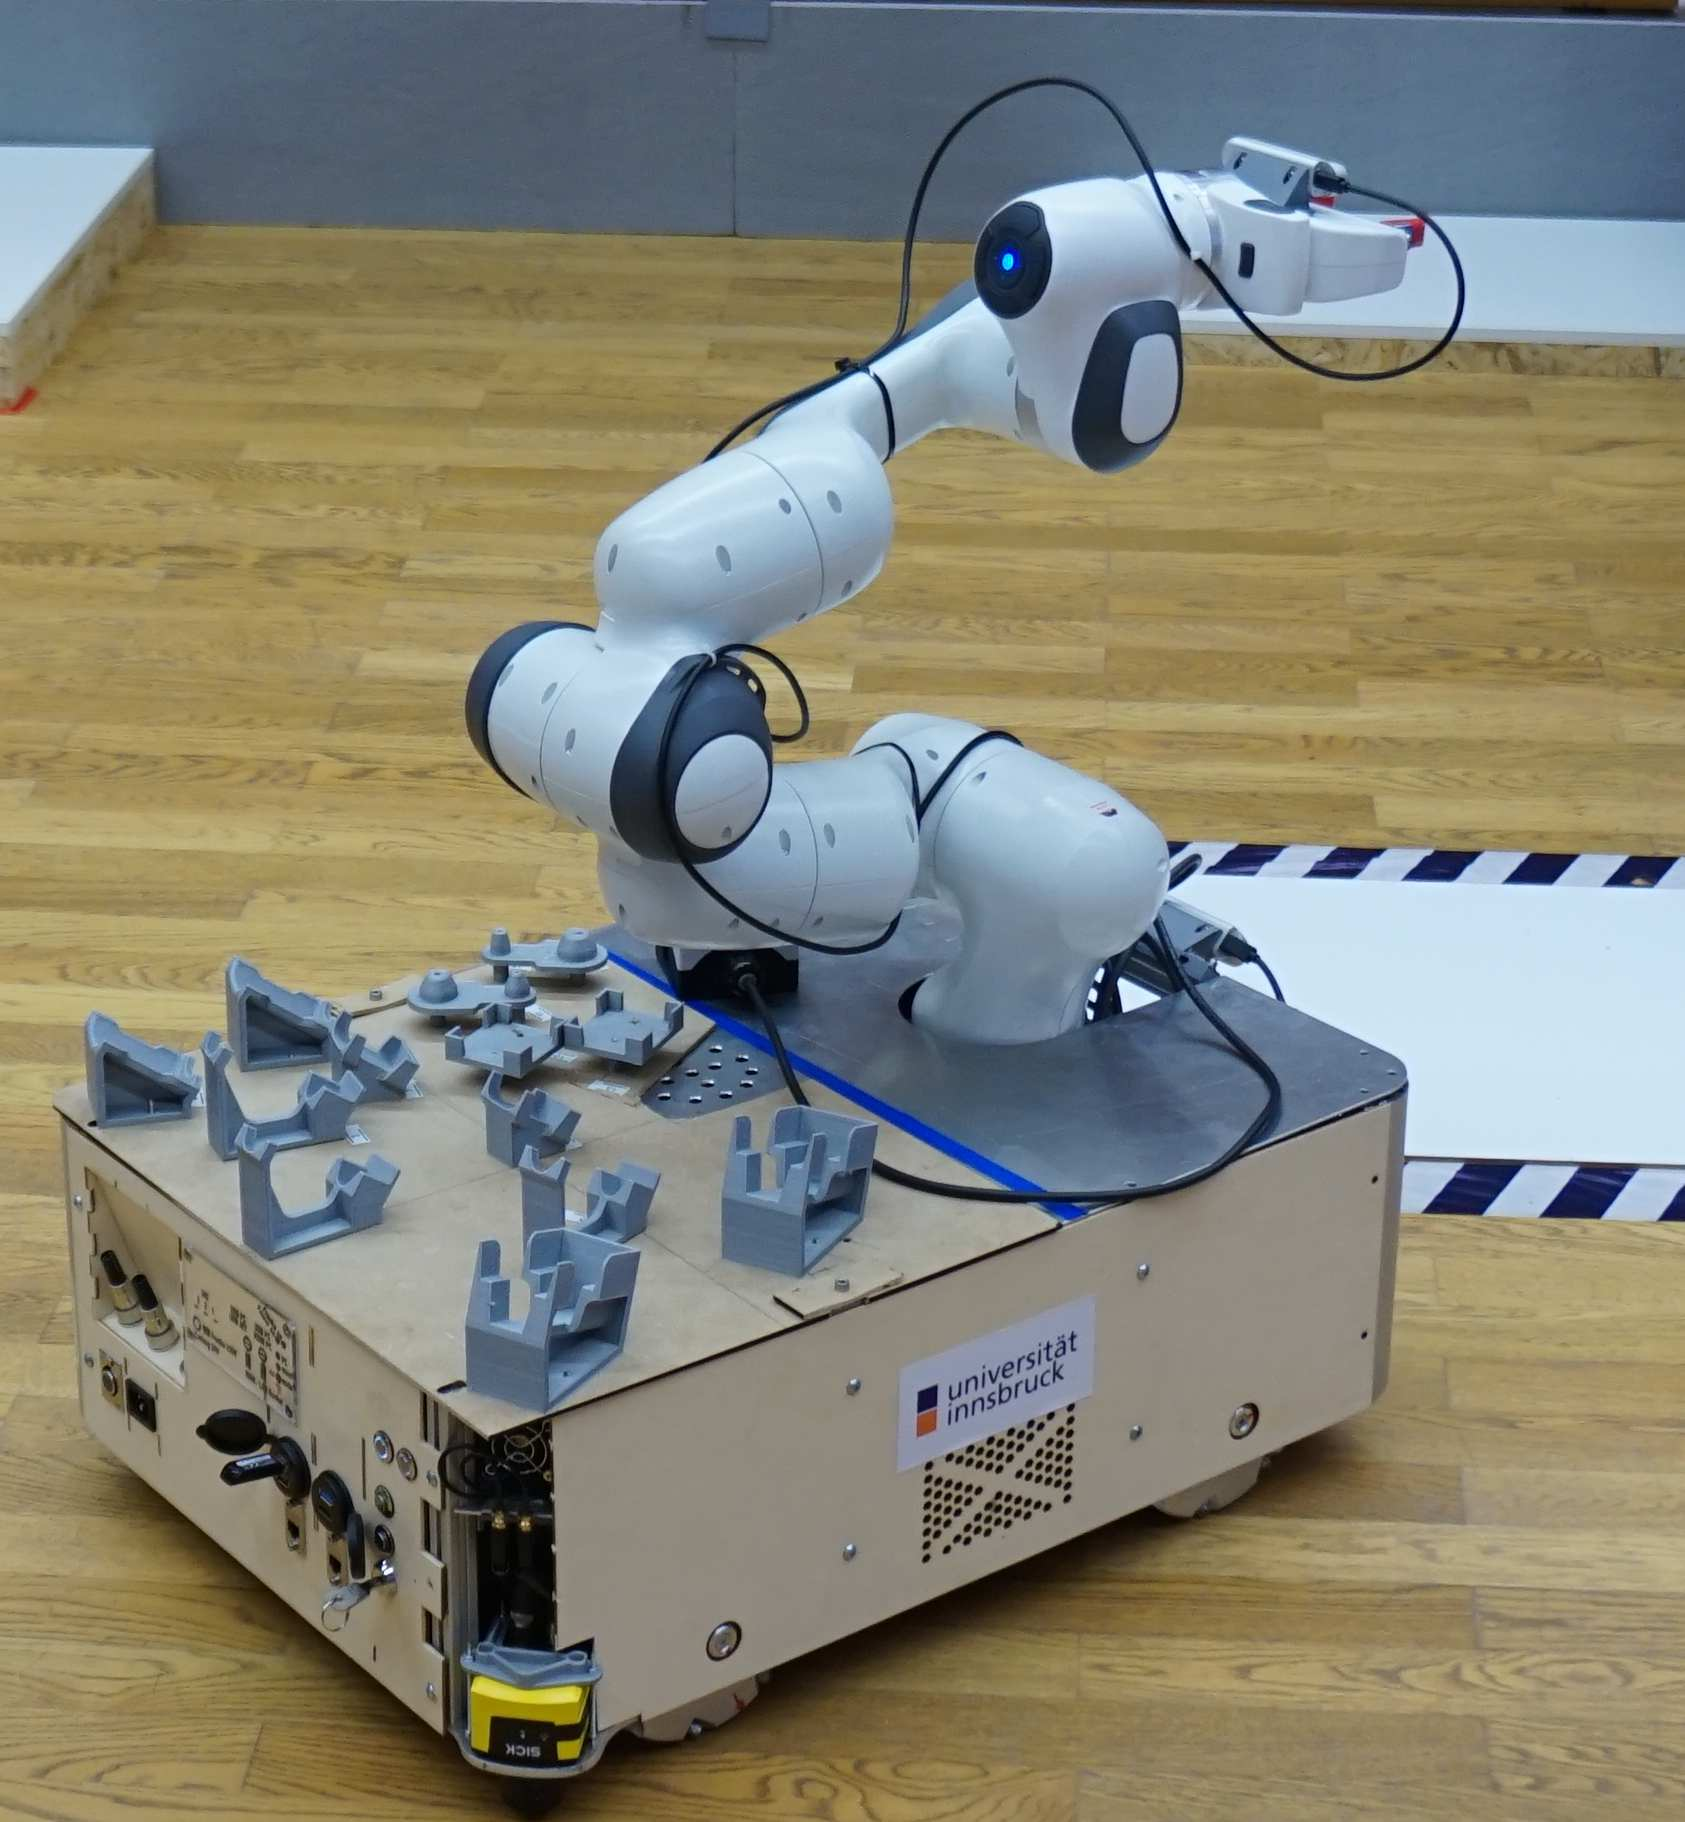
\includegraphics[width=0.31\textwidth]{./images/robots/tyrolics2.jpg}} \hfill
		\subfloat{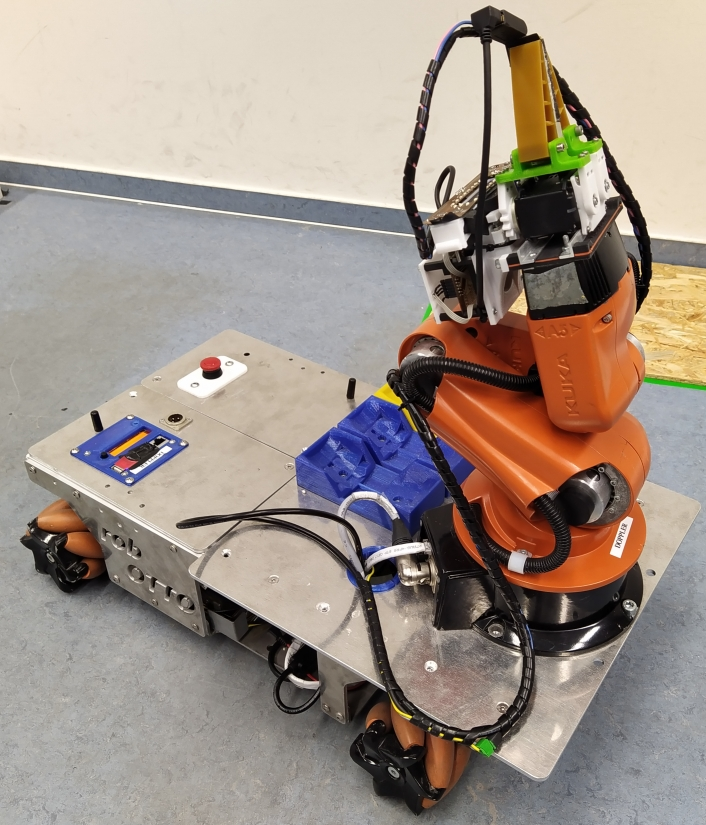
\includegraphics[width=0.3\textwidth]{./images/robots/robotto_bot_small.jpg}} 
	\end{center}
	\caption{Examples mobile robot platforms that can be used for \RCAW. Robots from the teams AutonOHM (Nuernberg-Germany), Tyrolics (Innsbruck-Austria) and robOTTO (Magdeburg-Germany) -- from left to right. }
	\label{fig:example_robots}
\end{figure}


\subsection{Behavior and Safety} \label{ssec:RobotBehaviorAndSafety}
For safety the robots have to meet the constraints in section \ref{ssec:RobotDesignAndConstraints}. In general, all robots shall be operated with maximum safety in mind. Any robot operation must be such that a robot neither harms humans nor damages the environment. 
The used batteries shall be handled with care and all team members must be educated in the correct usage, charging and storage of the batteries of the team. For lithium batteries appropriate storage bags must be used by the teams. The OC supplies a fire extinguisher for lithium batteries at the competition. If this is not sufficient for the used batteries of a team. The team is responsible for supplying an appropriate fire extinguisher by themselfs. The OC and TC control the observance of this rules.

All robots must have an emergency stop button. The emergency stop has to be a hard stop mechanism, that ensures that the energy transfer to all actuators is stopped immediately and the robot halts. The mechanism must be a red emergency stop button that is clearly visible, easily accessible and per wire attached to the robot. It has to be easy accessible from at least 3 sides of the robot. A wireless emergency stop button is optional but not sufficient.

The OC may request the proof of a robot's safety (e.g. the correct operation of an emergency stop) anytime during the competition and exclude teams that cannot satisfy safety requirements.

When participating in a competition, the team may operate the robot only in their own team area, in the arenas provided (possibly constrained by a schedule assigning periods of time for exclusive use of the arena by a team or a group of teams), and in any other areas designated by the organizers for robot operation. Any operation of robots outside of these areas, e.g. in public areas or emergency paths, require prior permission by the OC.

\textbf{Safety test procedure:}

Before the competition starts each robot has to perform a safety test procedure. This will be included in the competition schedule given by the OC.
\begin{itemize}
	\item Inspection of the robot platform (sharp edges and general construction)
	\item Description of the included safety systems by the team captain 
	\item Test of emergency stop while standing still
	\item Test of emergency stop while driving 
	\item Test of emergency stop while manipulation
\end{itemize}

\clearpage

\section{Arena Environment}
\label{sec:ArenaDesign}
The competition is held in an arena resembling an example layout of industrial manufacturing facilities. In this Section different parts of the environment are explained.
\subsection{General}
\label{ssec:ArenaGeneral}

%\textbf{Layout:}
The arena is a static 2D environment consisting of Walls, Tables and Obstacles etc. with a size of atleast 10 m$^2$ and not more than 120 m$^2$. 
An example layout is shown in fig. \ref{fig:arena_example}.

\begin{figure} [h!]
\centering
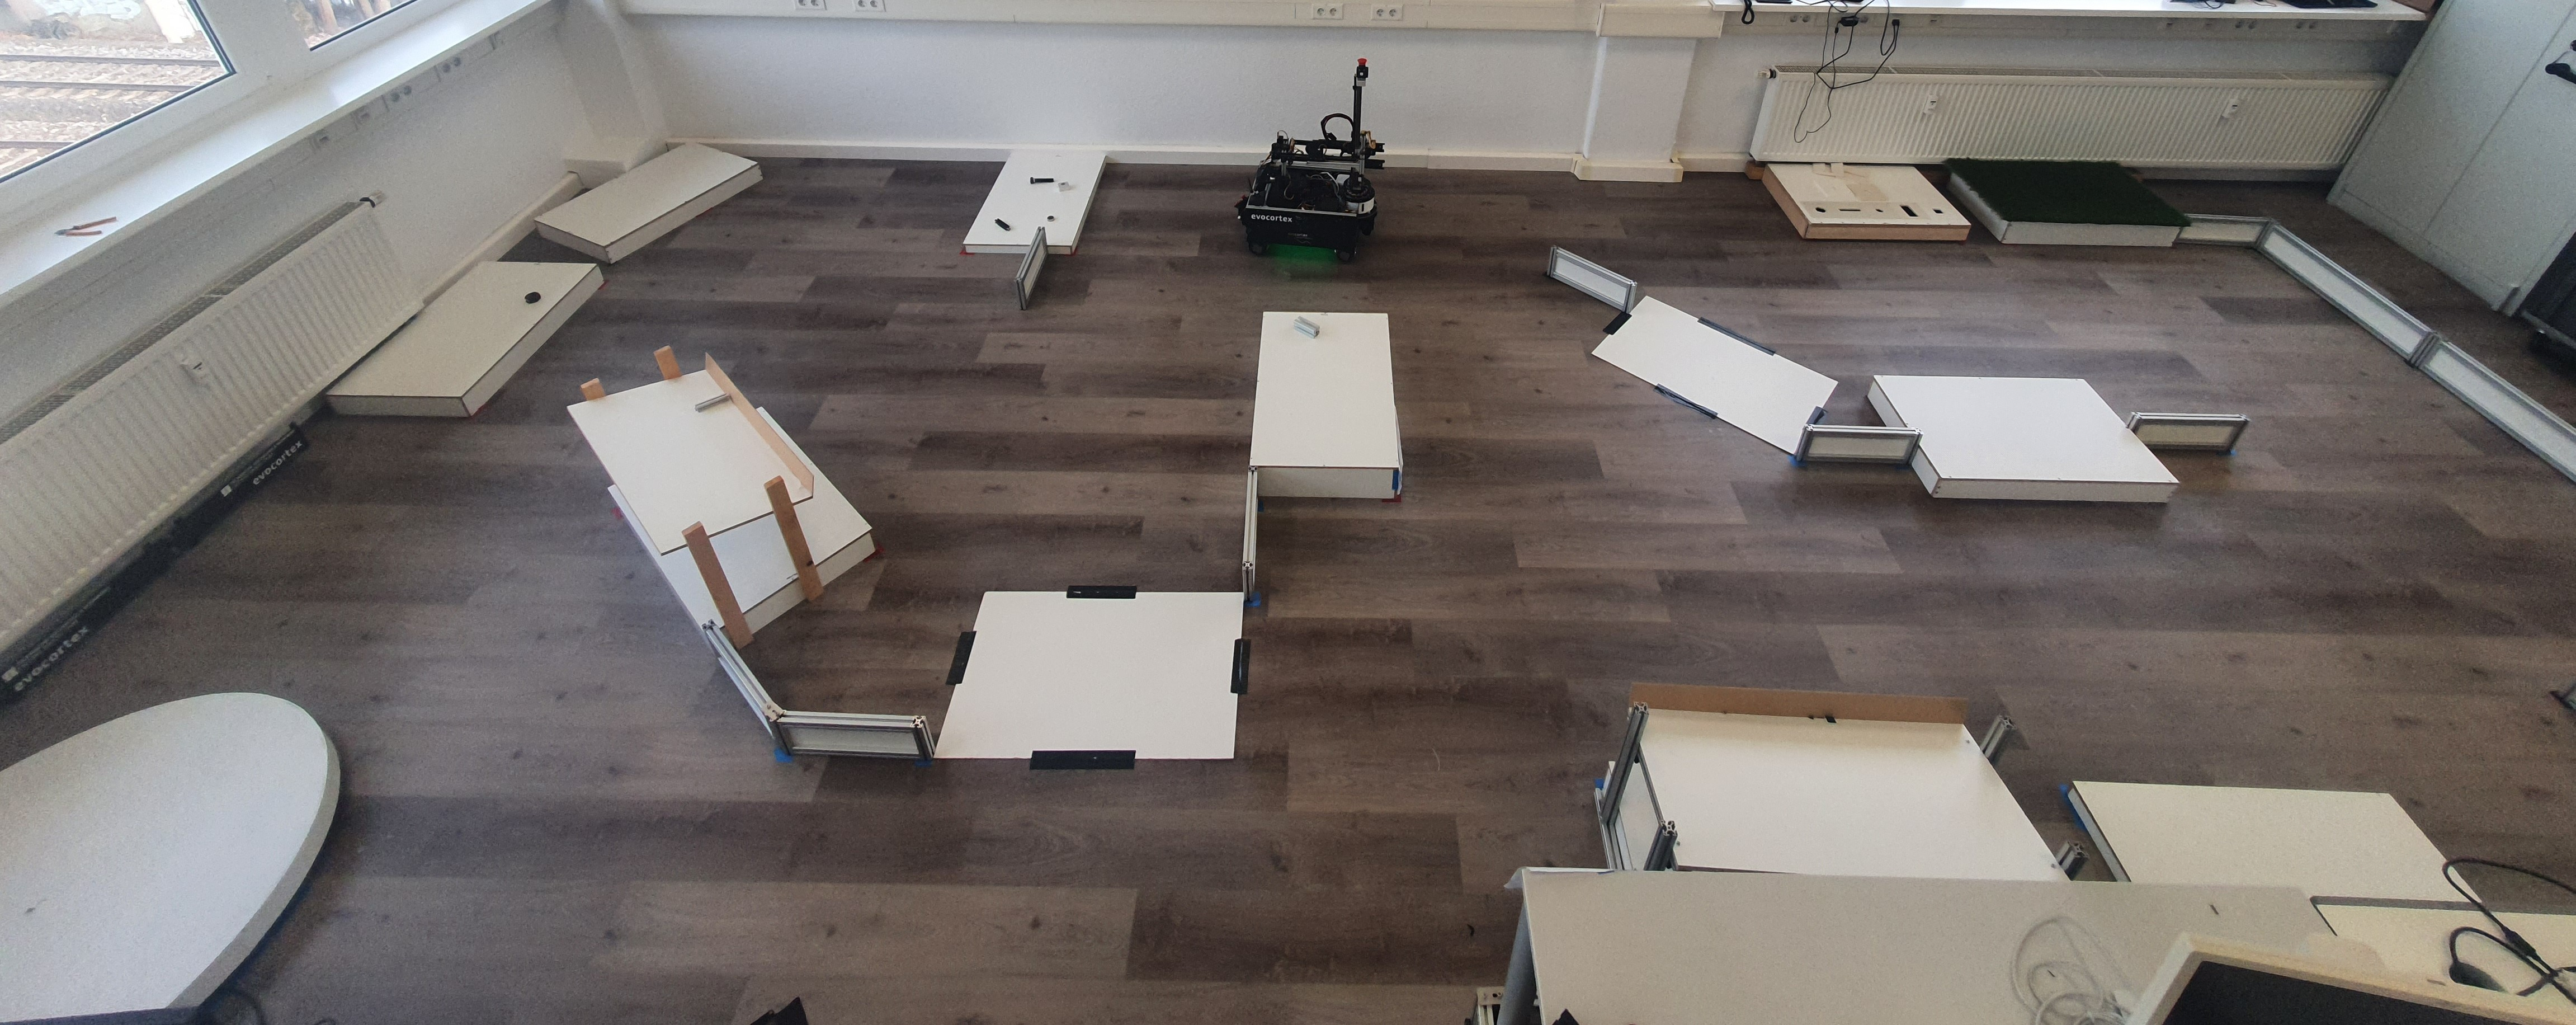
\includegraphics[width= 1\textwidth ]{./images/general_rules/arena_example.jpg}
\caption{An exemplary setup of a \RCAW environment.}
\label{fig:arena_example}
\end{figure}

Layouts may include rooms and hallways to create more realistic scenarios.
Service Areas (see section \ref{sec:Service_Areas}) mark the locations for robots to perform tasks.
Each requested Service Area must be accessible via atleast one path of $80\si{\centi\meter}$ width.

\textcolor{red}{Between the area where the robot is and where the spectators stand is the referee zone. The referee zone should allow the referees to move freely around the arena.}

\begin{figure} [h!]
\centering
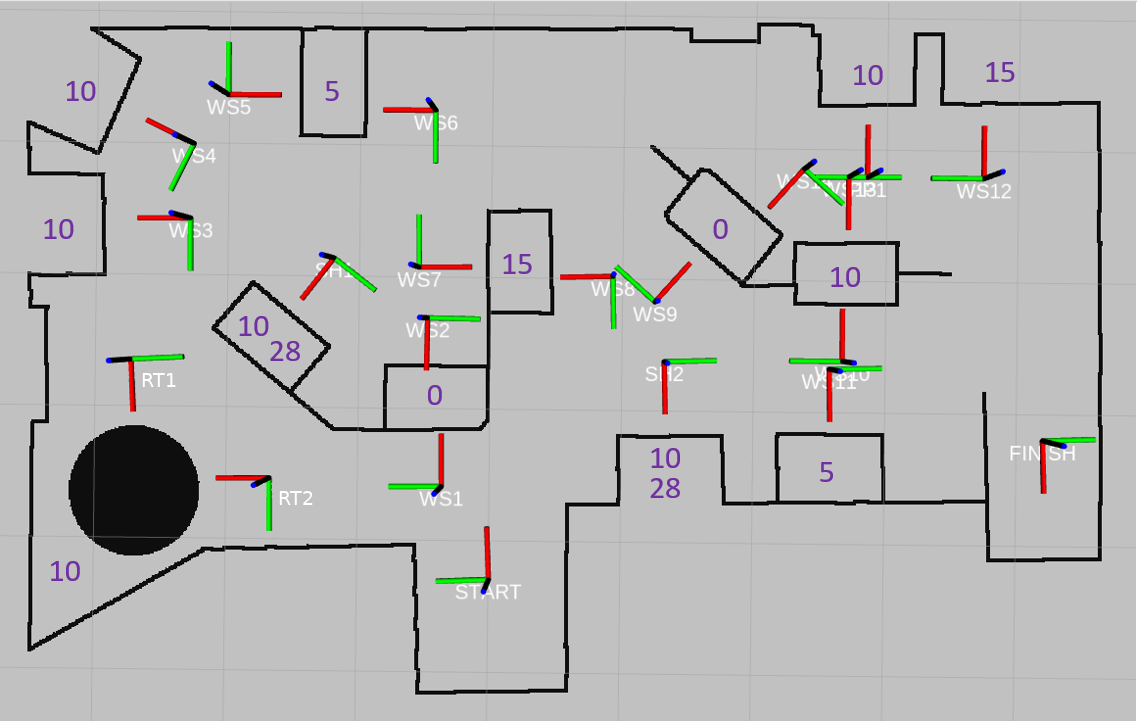
\includegraphics[width= 0.8\textwidth ]{./images/general_rules/arena_map_annotated}
\caption{Annotated 2D map of the environment in fig. \ref{fig:arena_example}}
\label{fig:arena_map_annotated}
\end{figure}

Each competition has a new and unique layout designed by the actual TC members.
It should feature:
\begin{itemize}
\item Area 10 m$^2$ - 120 m$^2$
\item Minimum distance between arena elements at least $80\si{\centi\meter}$ 
\item Widespread Service Areas entailing robot movements
\item Multiple paths between Service Areas
\item START and FINISH area
\end{itemize}


\textbf{START and FINISH area:}
\label{subsubsec: Start and Goal Area}

One or two parts of the arena are separated with marking Tape and considered as START and FINISH area. The START and FINISH area can be the same or two independent areas. The robot may leave the START area and enter the FINISH area only once. The START/FINISH area is leaved/entered when the robot completely cross the corresponding Marking Tape. In figure \ref{fig:tapeconfig} an exemplary Tape configuration is shown. As soon as the robot enters the FINISH area or re-enters the START area the run ends. The FINISH area counts as a Service Area and reaching the FINISH area gives additional points. 

\begin{figure} [h!]
	\begin{center}
		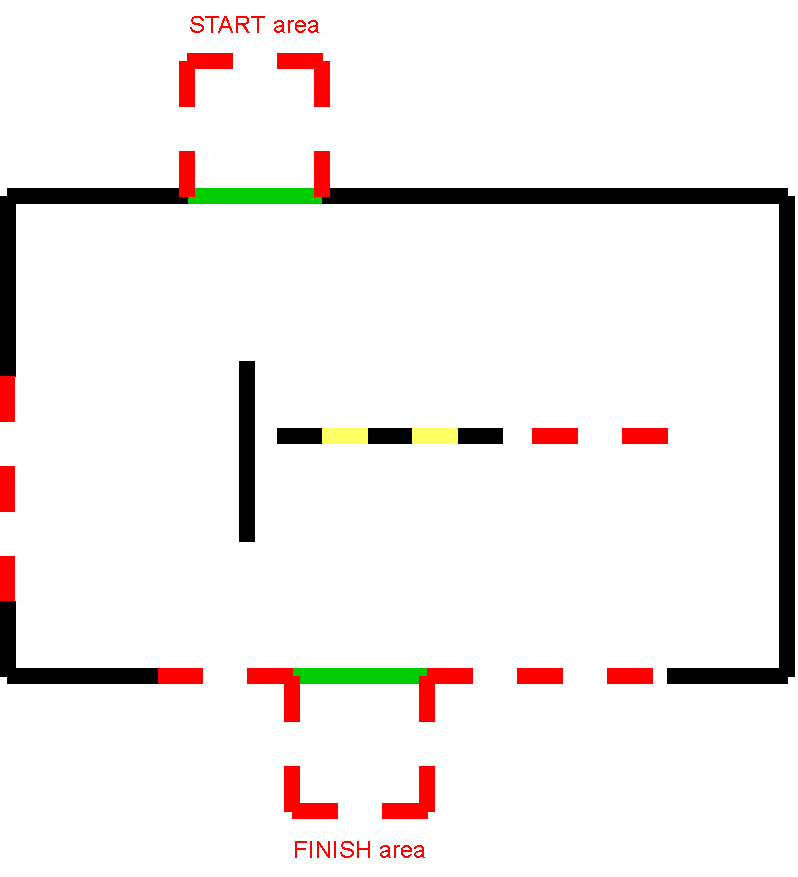
\includegraphics[width= 0.6\linewidth]{./images/arena/tabes.pdf}
	\end{center}
	\caption{Exemplary tape configuration: black lines are physical walls, red white dashed lines are virtual walls, yellow black dashed lines are barrier tape and green lines are marking tape}
	\label{fig:tapeconfig}
\end{figure}

\textbf{Floor}

The floor is made of some firm material. This includes among others floors made of concrete, screed, timber, plywood, chipboard, laminated boards, linoleum, PVC flooring, or carpet. Some examples are illustrated in Figure \ref{fig:example_floors}. Floors may neither be made of loose material of any kind (gravel, sand, or any material which may damage the functioning of the robot's wheels) nor may such material be used on top of the floor. Liquids of any kind are not allowed. The floor may have spots of unevenness of up to $1\si{\centi\meter}$ in any direction (clefts, rifts, ridges, etc.).


\begin{figure} [h!]
	\begin{center}
		\subfloat{
\includegraphics[height = 2cm]{./images/general_rules/example_floor_1.jpg}} \hspace{0.1cm}
		\subfloat{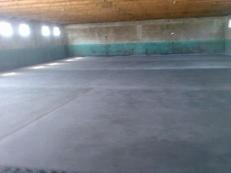
\includegraphics[height = 2cm]{./images/general_rules/example_floor_2.jpg}} \hspace{0.1cm}
		\subfloat{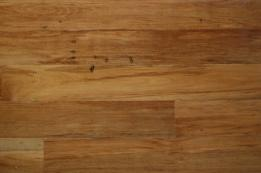
\includegraphics[height = 2cm]{./images/general_rules/example_floor_3.jpg}} \hspace{0.1cm}
		\subfloat{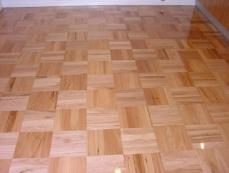
\includegraphics[height = 2cm]{./images/general_rules/example_floor_4.jpg}} \hspace{0.1cm}
		\subfloat{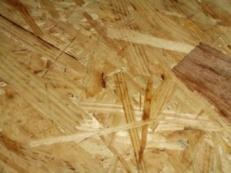
\includegraphics[height = 2cm]{./images/general_rules/example_floor_5.jpg}}\\
		\subfloat{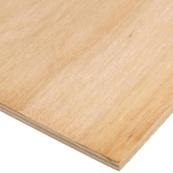
\includegraphics[height = 2cm]{./images/general_rules/example_floor_6.jpg}} \hspace{0.1cm}
		\subfloat{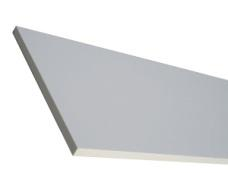
\includegraphics[height = 2cm]{./images/general_rules/example_floor_7.jpg}} \hspace{0.1cm}
		\subfloat{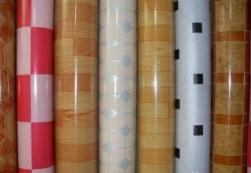
\includegraphics[height = 2cm]{./images/general_rules/example_floor_8.jpg}} \hspace{0.1cm}
		\subfloat{
\includegraphics[height = 2cm]{./images/general_rules/example_floor_9.jpg}} \hspace{0.1cm}
		\subfloat{
\includegraphics[height = 2cm]{./images/general_rules/example_floor_10.jpg}}
	\end{center}
	\caption{Examples of floors that can be used for \RCAW arenas.}
	\label{fig:example_floors}
\end{figure}





\subsection{Walls and Virtual Walls}
\label{subsec: Walls and virtual Walls}

The arena consists of outer and inner Walls used to build structures, create obstacles or function as protection barriers for teams and viewers. Walls may be either physical (plank) or virtual (red/white Tape). All walls (physical and virtual) have an infinitely height.
The arena is completely enclosed by Walls (both types possible), meaning robots are not allowed to exit the arena during a run. All types of Walls won't be changed during the competition. If the robot touches a Wall or Virtual Wall it results in a Major Collision.

The height of a physical Wall must be not less than $20\si{\centi\meter}$ and not more than $40\si{\centi\meter}$ (but will be seen as infinite high). Most Walls have a uniform main color (white), but may be enforced by metal (aluminum framework) and decorated with sponsor logos or ads.

Virtual Walls are made of red/white Tape and may never be crossed during a run. The arena can contain Walls and Virtual Walls inside.

\begin{figure} [h!]
\centering
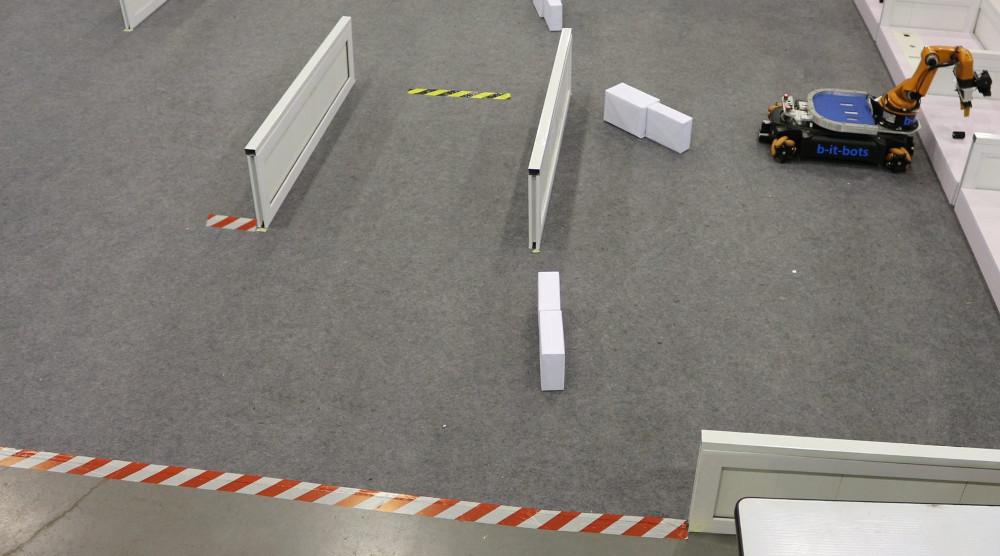
\includegraphics[width= 0.8\textwidth ]{./images/general_rules/barrier_tapes_in_china15.jpg}
\caption{Example of a typical arena. The red/white Tape indicates a Virtual Wall. The yellow/black Tape indicates a Virtual Obstacle and the white ashlar-formed cartonages are Obstacles.}
\label{fig:walls_and_virt_walls}
\end{figure}

\subsection{Obstacles}
\label{subsec: Obstacles}

In addition to the static arena elements, semi-dynamic Obstacles may be placed inside the arena before a competition run begins. 
The position of such Obstacles is decided by the TC during the setup phase of the run and randomized between different run types. Obstacles can be either physical or virtual.

Obstacles may block paths partly or completely, as long as all active Service Areas are still reachable.
There are three main Obstacle placement types:

\begin{itemize}
\item \textbf{Blocking:} 
A narrow section is completely blocked by the Obstacle, which means that no robot can physically pass it ($<$ $20\si{\centi\meter}$).

\item \textbf{Semi-Blocking:} 
The Obstacle reduces the distance between arena elements below the minimum width for a path ($<$ $80\si{\centi\meter}$). The path therefore counts as blocked, meaning that there must exist another valid path to all active Service Areas. Robots are still allowed to use all paths if they fit through the smaller gaps.
The gap width is fixed and its value is calculated using the width of the biggest robot in the competition plus $ 10\si{\centi\meter}$. This usually adds up to around $ 60\si{\centi\meter}$,
but might be higher or lower, depending on the participating robots.

\item \textbf{Non-Blocking:}
The Obstacle adds or enlarges an arena element but keeps all paths intact.
\end{itemize}


Physical Obstacles (see figure \ref{fig:walls_and_virt_walls}) measure atleast $2\si{\centi\meter}$ x $2\si{\centi\meter}$ x $20\si{\centi\meter}$ (l x w x h) and may be made of any non-transparent, firm material (wood, metal). Some examples are bins, shipping boxes and Wall elements. Their color is not specified.
All physical Obstacles are treated like any other arena element during a run, including the rules for collisions (Major Collision).

Virtual Obstacles are marked using the yellow/black Tape from section \ref{subsec:Tapes}. The collisions with these Virtual Obstacles will treated as Tape Collision (see \ref{sec:penalties}).


\subsection{Tapes}
\label{subsec:Tapes}

\textbf{Red/white Tape:}

The red/white Tape (Tesa signal $5\si{\centi\meter}$ width) is considered as a Virtual Wall and has an infinite height. The red/white Tape is static and won't be changed during the whole competition. It will be used inside the arena and as an outer border of the arena.  Touching the red/white Tape is considered as a Major Collision.

\textbf{Yellow/black Tape:}

The yellow/black Tape (Tesa signal $5\si{\centi\meter}$ width) is considered as a Virtual Obstacles and has an infinite height. The yellow/black Tape will be placed by the TC before a run that contains Virtual Obstacles. Touching the yellow/black Tape is considered as a Tape Collision.

\begin{figure} [h!]
	\centering
	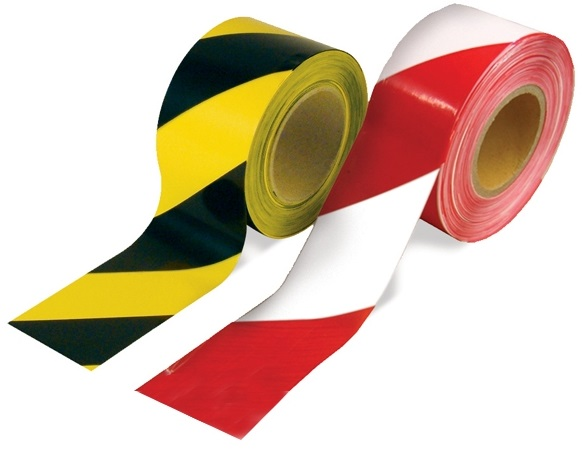
\includegraphics[width= 0.4\textwidth ]{./images/general_rules/example_barrier_tape}
	\caption{Example red/white and yellow/black Tapes}
	\label{fig:tapes}
\end{figure}

\textbf{Markup Tape:}

Green electrical tape is considered as markup Tape. This tape can be used everywhere, where it is useful. It is intended as a marker for the referees and teams and not for the robot. Therefore the color may deviate, but the color is not red or yellow to guarantee a clear difference to the other tapes. The tape is used to mark the START and FINISH area. Furthermore the tape can be used to mark the position of tables (especially $0\si{\centi\meter}$) and Walls. The latter ones are useful for restoring the arena in case of a Major Collision.


\subsection{Tables}
\label{subsec: Tables}

%52. However, from 2020 on and in order to make the competition more realistic, the heights of the Tables will be variable, allowing the OC to adjust them before each test run.-> No???
%-> every height of the Tables can have a margin of $2\si{\centi\meter}$
%-> Table height “fixed”, but may change due to Arbitrary Surface (margin of $2\si{\centi\meter}$)
%Leander

%54. Define Table Size:
%-> 80cm x 50cm x X cm (0, 5, 10, 15)
%-> same size for shelf
%Leander

%However, from 2020 on and in order to make the competition more realistic, the heights of the service Areas will be variable, allowing the OC to adjust them before each test run. TODO...

Tables normally used have a width (the side the robot approaches) of $80\si{\centi\meter}$ and a depth of $50\si{\centi\meter}$. In general terms, the table shall be big enough to contain at least one manipulation zone as described in section \ref{ssec:ManipulationZone}. In general two manipulation zones are included on one table (one zone on each side of the Table). The used table heights are $0\si{\centi\meter}$, $5\si{\centi\meter}$, $10\si{\centi\meter}$ and $15\si{\centi\meter}$. See further down in this section for more information about the $0\si{\centi\meter}$-Table. See figure \ref{fig:ws} for illustration. 
The tolerance for the heigth is $\pm 2 \si{\centi\meter}$. During a competition the Table size is only fixed in the margin of $\pm 2 \si{\centi\meter}$, because of arbitrary surfaces (see \ref{subsec:Arbitrary_Surfaces_and_Decoys} for an explanation of arbitrary surfaces). 
The table is closed between the bottom and the table top. That's why the Table can be used as a reference for navigation, when the height is sufficient for the robot. Note that the height may change slightly with arbitrary surfaces during a competition and thus the table can sometimes be visible to the laser scanners and sometimes not. 
 
\begin{figure} [h!]
	\begin{center}
		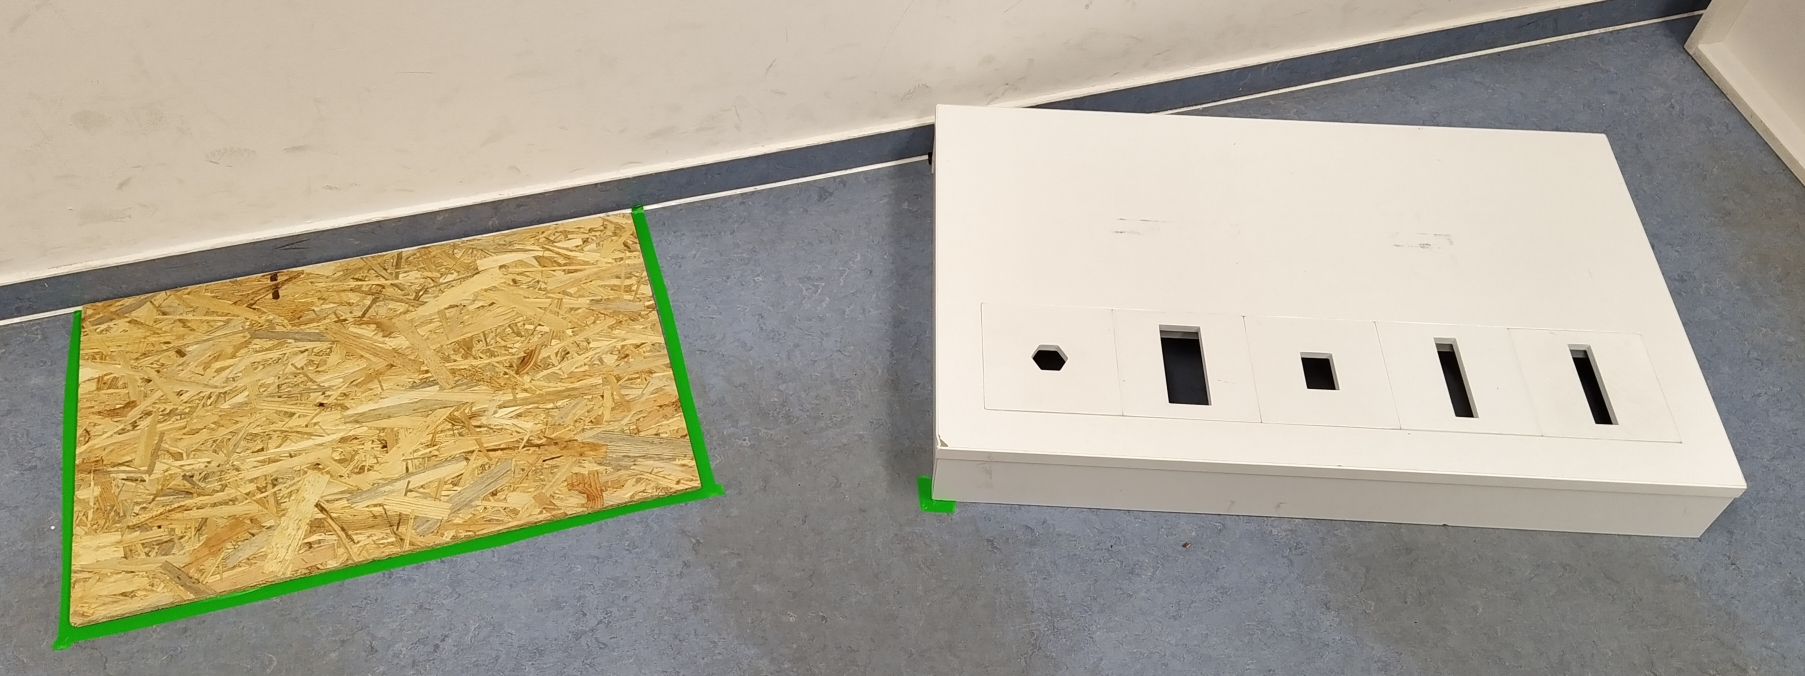
\includegraphics[height = 4cm]{./images/arena/tables_small.jpg}	
	\end{center}
	\caption{left: 0\si{\centi\meter}-Table with arbitrary surface (approx. 1\si{\centi\meter} thick); right: PPT-Table which is a standard 10\si{\centi\meter}-Table with cavities}
	\label{fig:ws}
\end{figure}

If a table has a height of $0\si{\centi\meter}$, a green electrical Tape (see \ref{subsec:Tapes}) will mark the area. A $0\si{\centi\meter}$-Table can be active or inactive. Active means, that the current test (see table \ref{tab:Instances}) includes $0\si{\centi\meter}$-Tables.
If the table is active, the surrounded area may be covered by a white sheet of paper or arbitrary surface. The material is not fixed.
The OC is responsible to replace it in case of pollution or tears. To reduce the tear, it is removed when the $0\si{\centi\meter}$-Table is not active. If the floor is white or the table shall have an Arbitrary Surface, no cover needs to be installed.
$0\si{\centi\meter}$-Table may be crossed and does not count as a collision. If the laid out white Surface is moved, it is not a collision.
If the robot touches an Object while navigating, this will be handled as a Minor Collision. Examples for $0\si{\centi\meter}$-Table are shown in figure \ref{fig:0cmws}.



\begin{figure} [h!]
		\begin{center}
			\subfloat{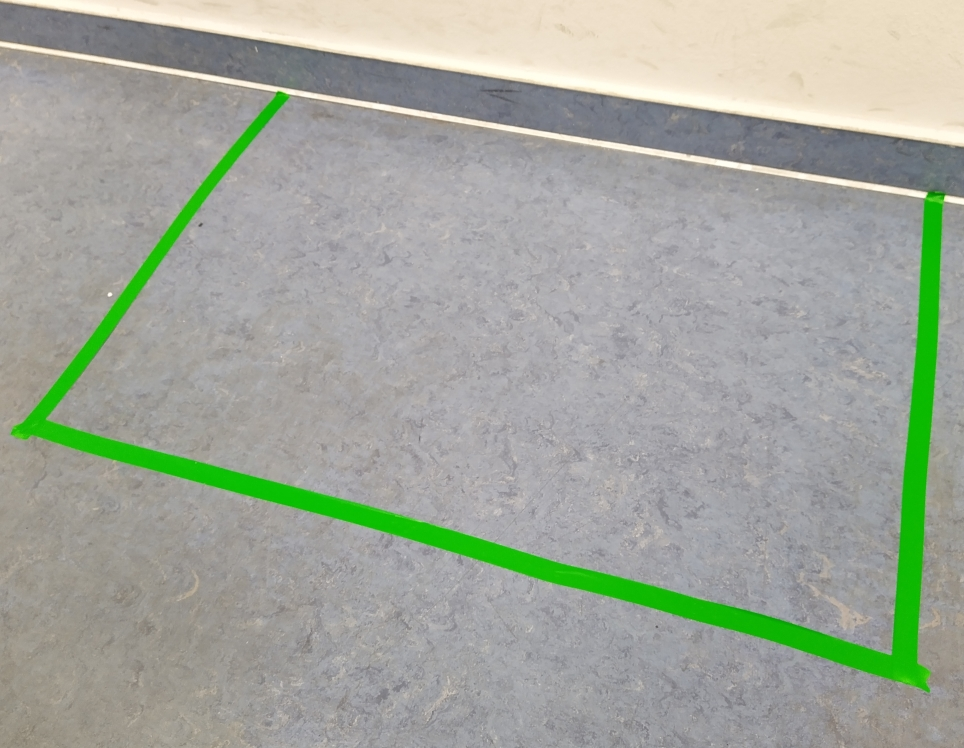
\includegraphics[width=0.4\textwidth]{./images/arena/table_0_inactive_small.jpg}} \hspace{0.2cm}
			\subfloat{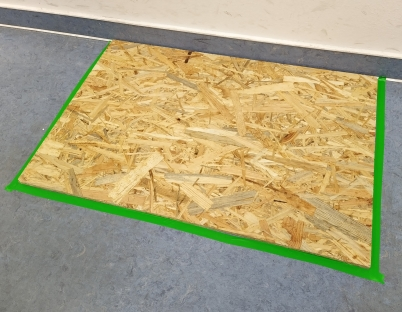
\includegraphics[width=0.4\textwidth]{./images/arena/table_0_arb_small.jpg}} 
		\end{center}
	\caption{left: $0\si{\centi\meter}$-Table which is considered as inactive or as an active table with arbitrary surface; right: $0\si{\centi\meter}$-Table which is considered as active with an arbitrary surface}
	\label{fig:0cmws}
\end{figure}

\subsection{Shelves}\label{sec:Shelves}

The integration of Shelves into tests is according the table \ref{tab:Instances}. Service Areas may foresee the use of shelves and shelf units as depicted in Figure~\ref{fig:shelf}. The lower part of the Shelf is a $10\si{\centi\meter}$-Table as specified in \ref{subsec: Tables}.
The maximum height of the shelves should be not more than $40\si{\centi\meter}$. In the example shown in Figure~\ref{fig:shelf} the first $15 \si{\centi\meter}\pm 2\si{\centi\meter} $ are not covered by the top shelf. The length of free space can be changed during competition and can not be seen as mandatory. Therefore all teams has to consider special picking behavior to avoid collision.  

The top shelf surface may be specially designed in order to serve specific purposes, e.g.\, holding Objects. Objects for grasping are always placed on the bottom shelf. The placement of a delivered Object has to be done on the top shelf.  

\begin{figure}[h!]
	\centering
	\subfloat[A shelf with two levels and uniform colored surfaces.]{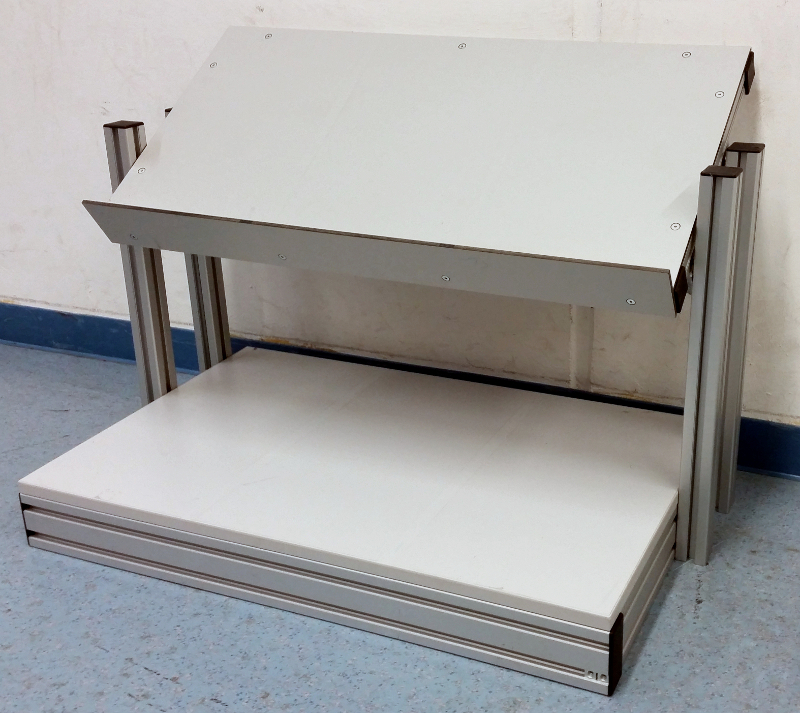
\includegraphics[width=0.375\textwidth ]{./images/shelf.jpg}}
	\hspace{0.05\textwidth}
	\subfloat[Technical draw of shelf configuration.]{ 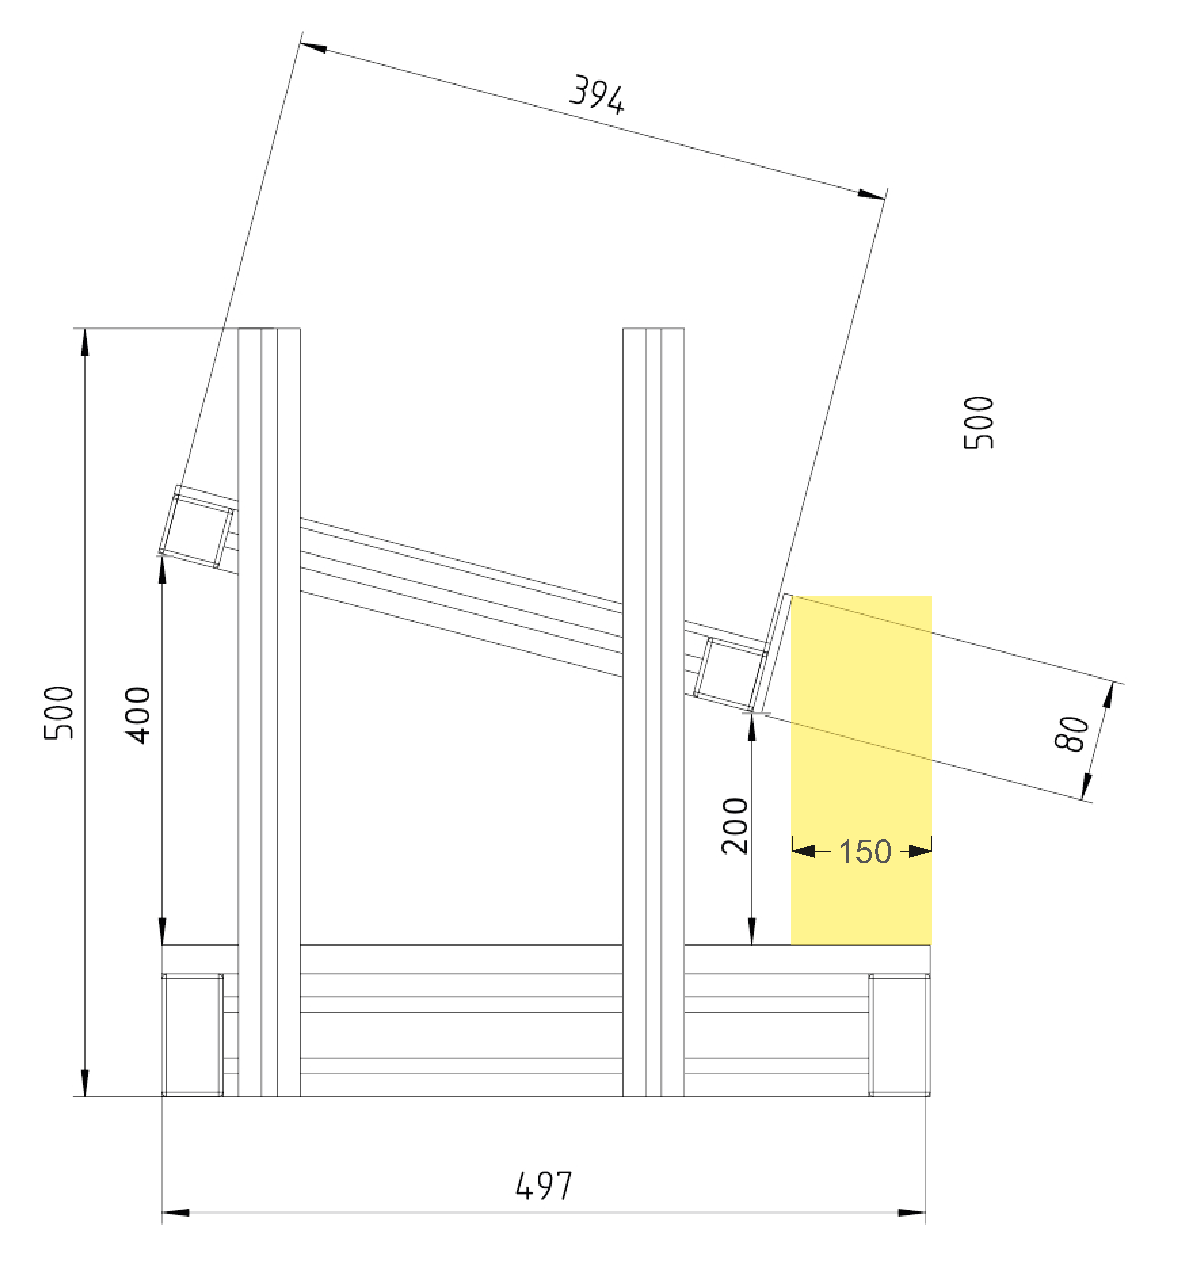
\includegraphics[width=0.375\textwidth ]{./images/shelfUpdate.pdf} }
	\caption{Exemplary shelf and generic technical drawing.}%
	\label{fig:shelf}
\end{figure}


\subsection{Rotating Tables}\label{sec:Rotating Table}
The integration of Rotating Tables into tests is according the table \ref{tab:Instances}.  A Rotating Table as depicted in Figure~\ref{fig:rottable} is used for these tests. The Objects placement is the same like in section \ref{ssec:ManipulationZone}, so the maximal depth for Objects is $20 \si{\centi\meter}$ and there is gap of $2\si{\centi\meter}$ to the border of the Rotating Table.


The height of the Rotating Table should be not lesser than $8\si{\centi\meter}$ and not be more than $12\si{\centi\meter}$. The diameter of the Rotating Table should be not lesser than $50\si{\centi\meter}$ and not more than $100\si{\centi\meter}$. The Rotating Table has to have a white surface colour. The rotating speed of the table depends on the diameter so that the Objects speed is able to vary between $5 \si{\centi\meter\per\second} \le v_{object} \le 20 \si{\centi\meter\per\second}$. This has to be adjusted by the referees before a team starts its run to a fixed value (some small variations in boarders of  technical feasibility are allowed). This is changed after each run type to another random chosen value in this range. During the run of a team the speed is static and each team will have the same table speed. Example: For a Rotating Table with diameter $d_{table}=1\si{\meter}$, Objects are placed on a grasp region with the diameter $d_{object}=0.8\si{\meter}$ with $\omega_{table} = \frac{2 \cdot v_{objects} }{d_{grasp}}=\frac{2 \cdot 0.2}{0.8}=0.5\si{\radian\per\second}$ and with $n_{table}=\frac{\omega_{table}}{2 \cdot \pi}=\frac{0.5}{2 \cdot \pi}$ the minimum rotational speed of the Rotating Table $n_{table}= 0.0796 \si{\per\second}$ (rounds per second) can be calculated.  

\begin{figure}[h!]
	\centering
	\subfloat[A Rotationg table with some Objects.]{%
		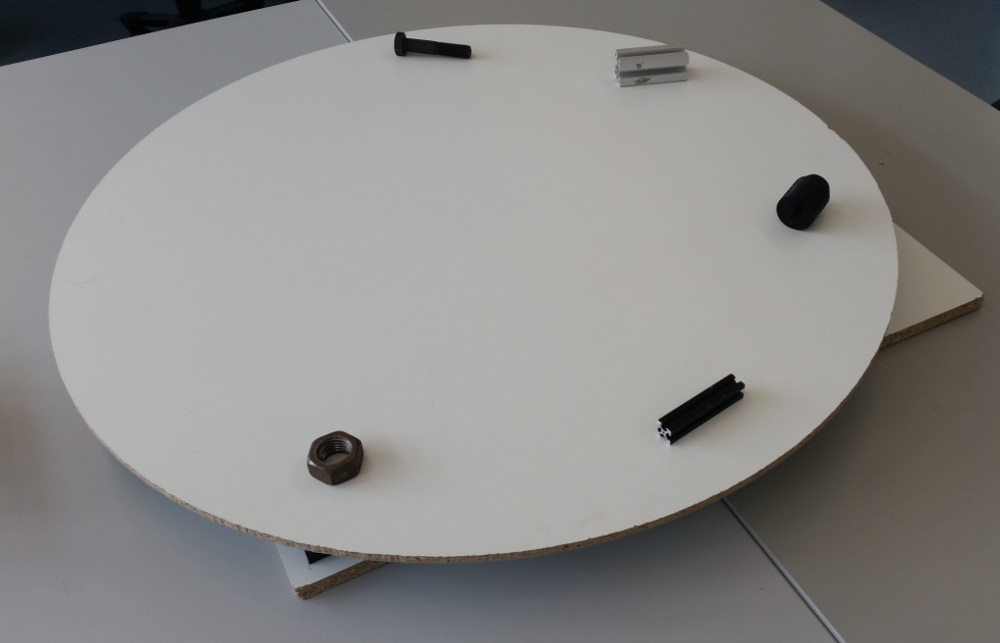
\includegraphics[width=0.375\textwidth,angle=0 ]{./images/rotating_table.jpg}%
	}%
	\hspace{0.05\textwidth}
	\subfloat[Technical draw of Rotating table.]{%
		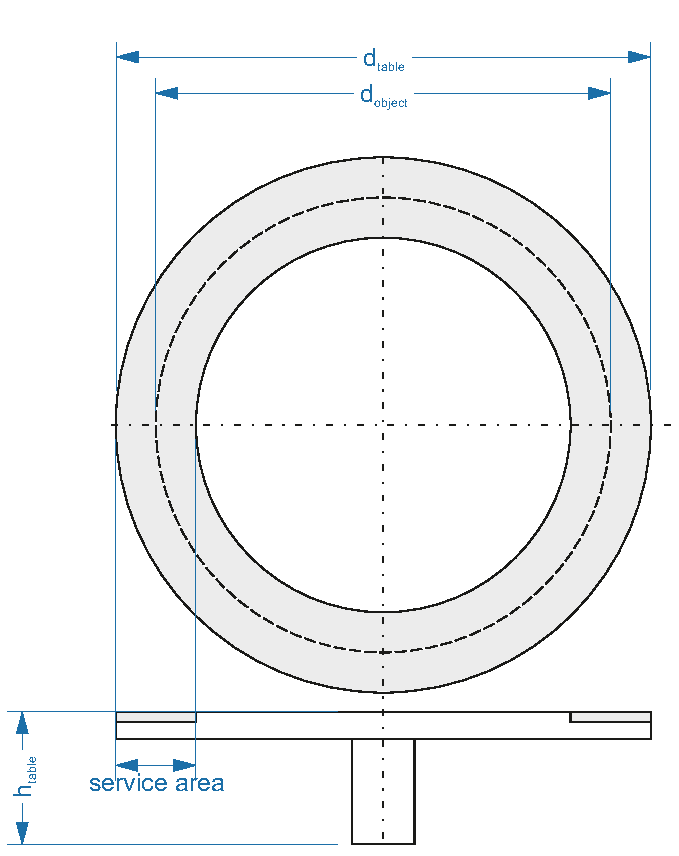
\includegraphics[width=0.375\textwidth ]{./images/rotating_table_schematic.pdf}
	}
	\caption{Exemplary Rotating table and generic technical drawing.}%
	\label{fig:rottable}
\end{figure}


\subsection{Precision Placement Tables}\label{sec:Precision Placement}

The precision placement table as shown in Figure~\ref{fig:ppt_table} includes object-specific cavities tiles as shown in the Figure~\ref{fig:ppt_tiles}. It is based on a standard $10\si{\centi\meter}$ table described in Section~\ref{subsec: Tables}. For each object used in the test, there will be one specific cavity. The cavity has the dimension of the object plus a $2 \si{\milli\meter}$ offset for each dimension. At most five cavities are used in the test. The cavities are in an random order on the table and are located within the standard manipulation zone defined in Figure~\ref{fig:manipulation_zone}. One cavity tile has the dimensions of $140 \si{\milli\meter} \times 140 \si{\milli\meter} $. Placing five cavities on a standard $10\si{\centi\meter}$ table leaves a boarder of $5 \si{\centi\meter}$ on each side of the table. The additional decoy cavity tiles will be chosen by the referees. For the Precision Placement Table only the RoboCup@Work Object Set will be used.

\begin{figure} [h!]
	\begin{center}
		\subfloat[F20\_20]{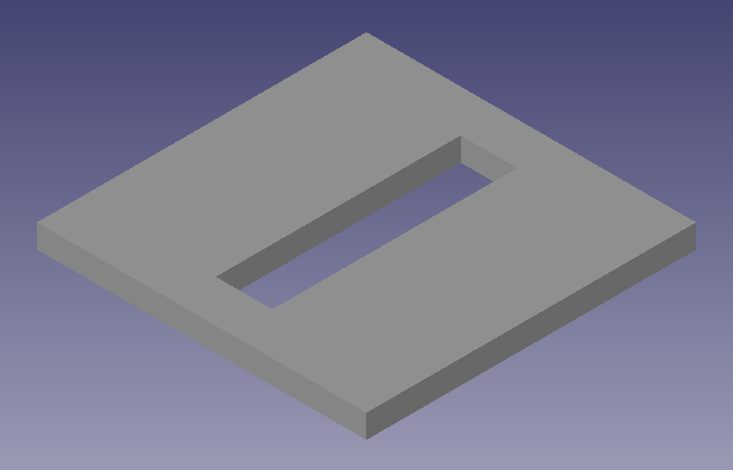
\includegraphics[width = 2cm]{./images/ppt_F20.png}} \hspace{0.1cm}
		\subfloat[S40\_40]{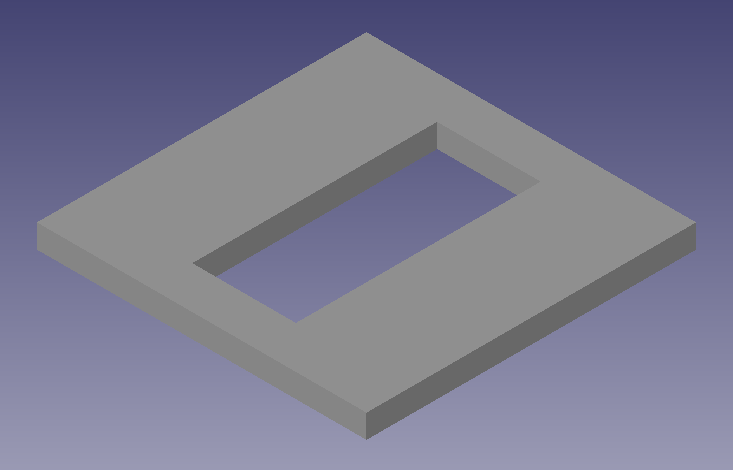
\includegraphics[width = 2cm]{./images/ppt_S40.png}} \hspace{0.1cm} 
		\subfloat[M20\_100]{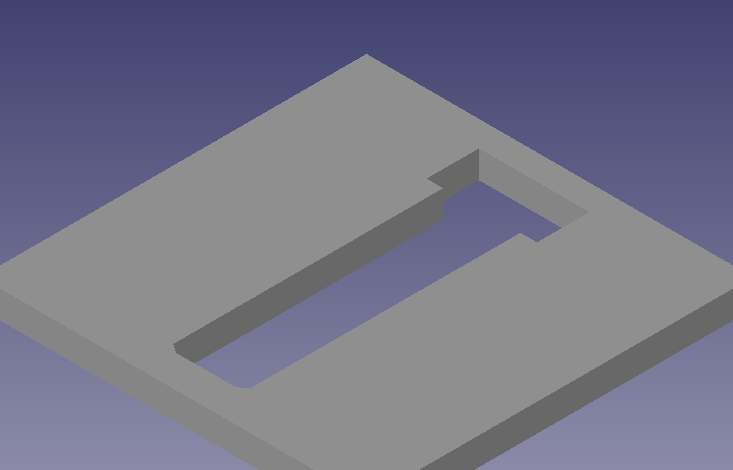
\includegraphics[width = 2cm]{./images/ppt_M20_100.png}}  \hspace{0.1cm}
		\subfloat[M20]{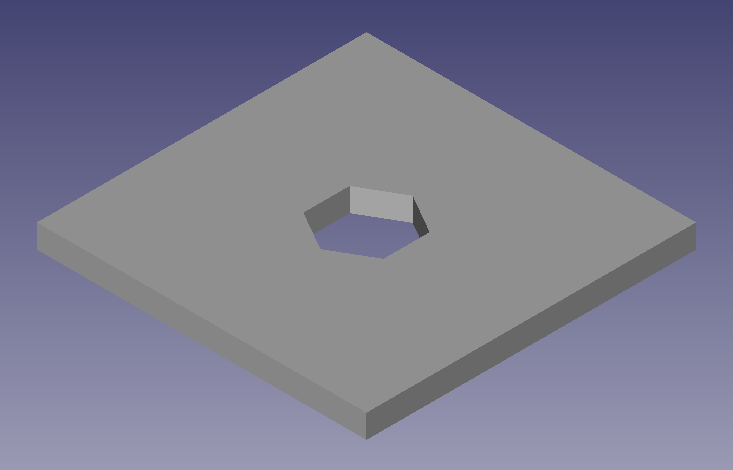
\includegraphics[width = 2cm]{./images/ppt_M20.png}}  \hspace{0.1cm}
		\subfloat[M30]{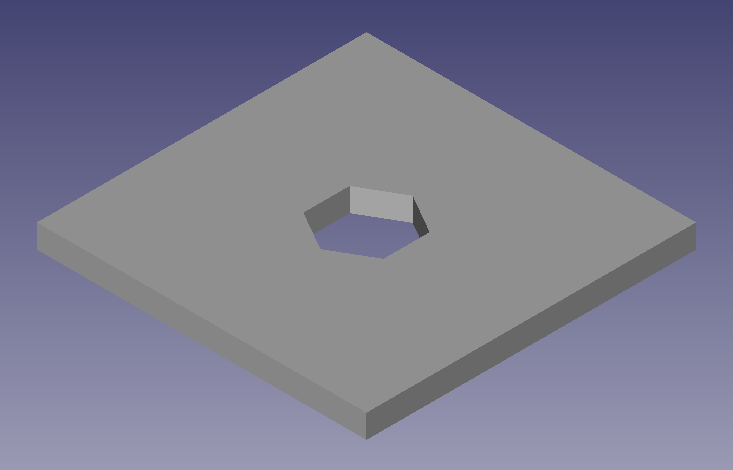
\includegraphics[width = 2cm]{./images/ppt_M30.png}}  \hspace{0.1cm}
		\subfloat[R20]{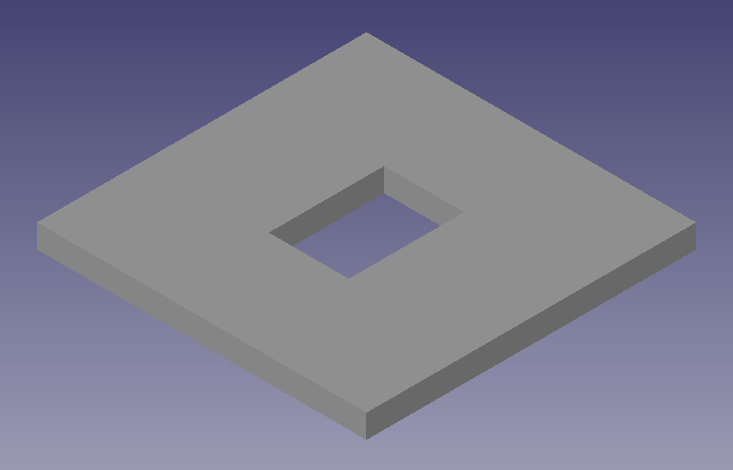
\includegraphics[width = 2cm]{./images/ppt_VR20.png}} \\
		\subfloat[F20\_20]{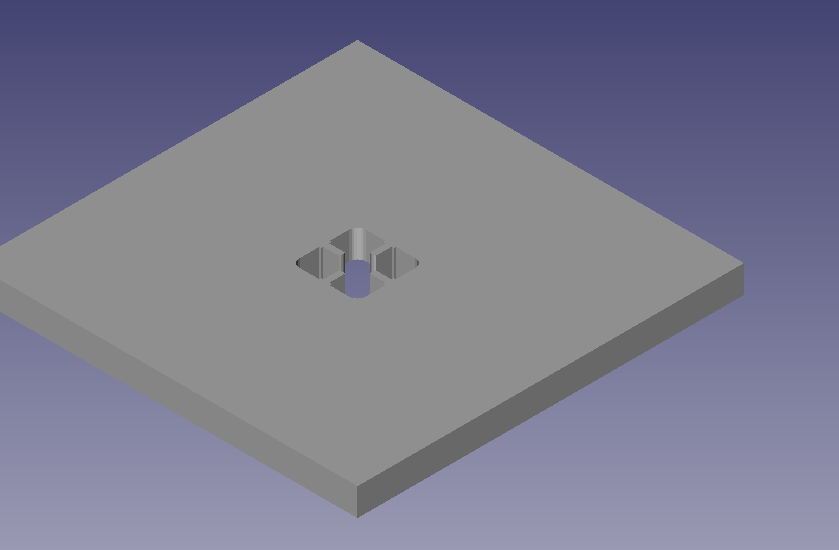
\includegraphics[width = 2cm]{./images/ppt_F20_v.png}}  \hspace{0.1cm}
		\subfloat[S40\_40]{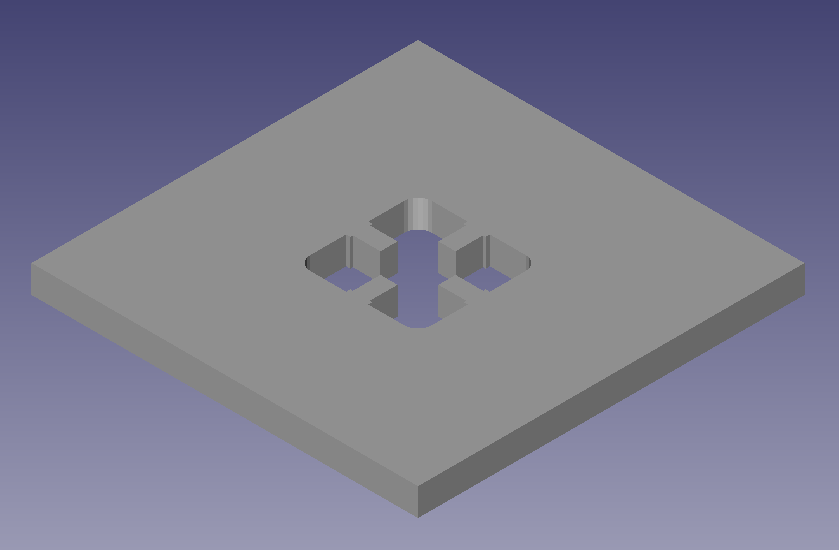
\includegraphics[width = 2cm]{./images/ppt_S40_v.png}}   \hspace{0.1cm}
		\subfloat[M20\_100]{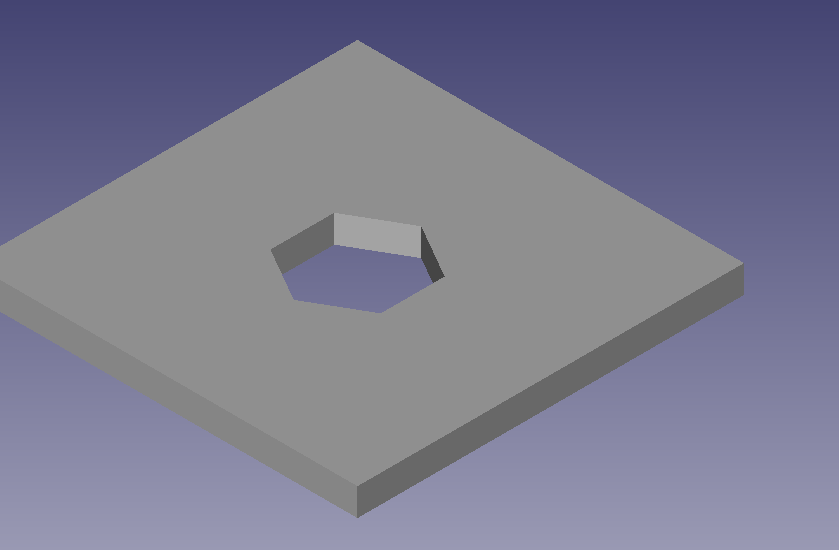
\includegraphics[width = 2cm]{./images/ppt_M20_100_v.png}} \hspace{0.1cm}
		\subfloat[M20]{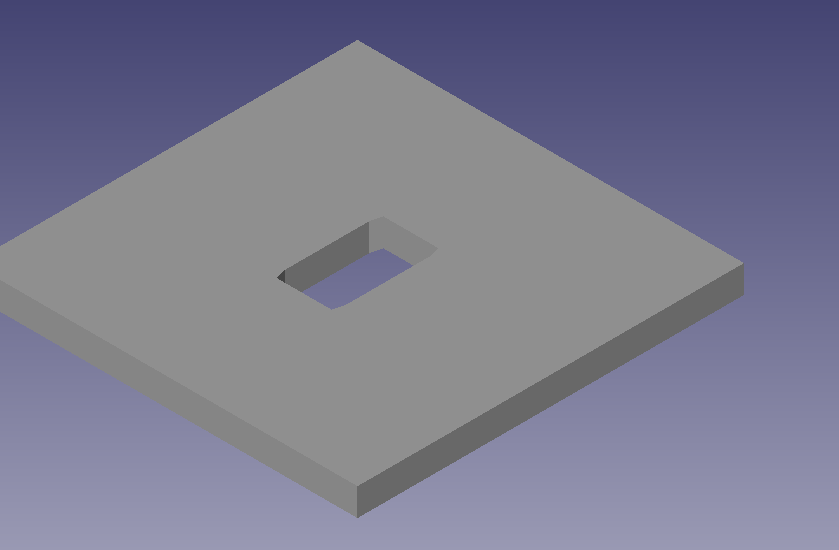
\includegraphics[width = 2cm]{./images/ppt_M20_v.png}}  \hspace{0.1cm}
		\subfloat[M30]{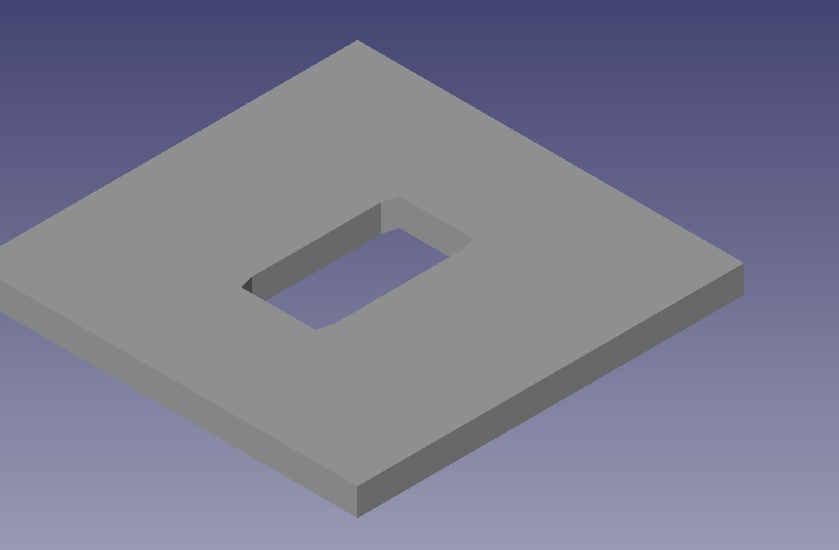
\includegraphics[width = 2cm]{./images/ppt_M30_v.png}}  \hspace{0.1cm}
		\subfloat[R20]{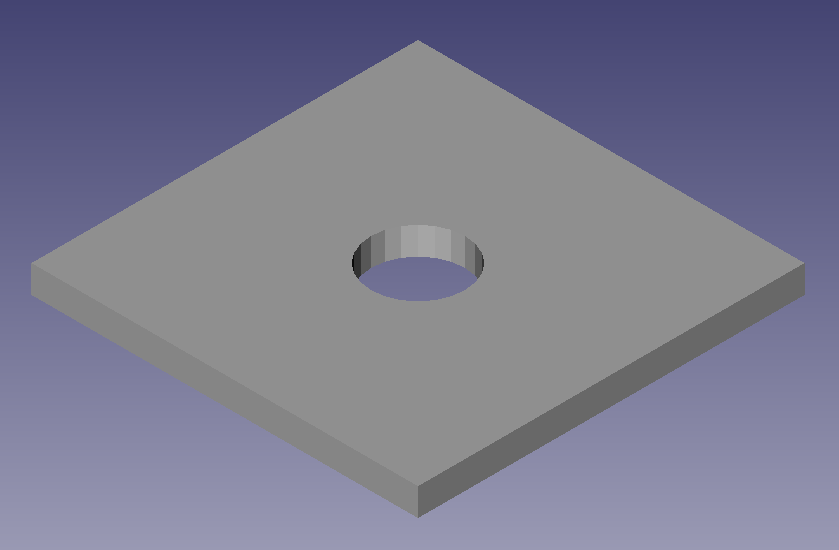
\includegraphics[width = 2cm]{./images/ppt_VR20_v.png}} 
	\end{center}
	\caption{Illustration of horizontal (top row) and vertical (bottom row) cavities for the different kind of manipulation objects.}
	\label{fig:ppt_tiles}
\end{figure}



%\begin{figure} [h!]
%	\centering
%	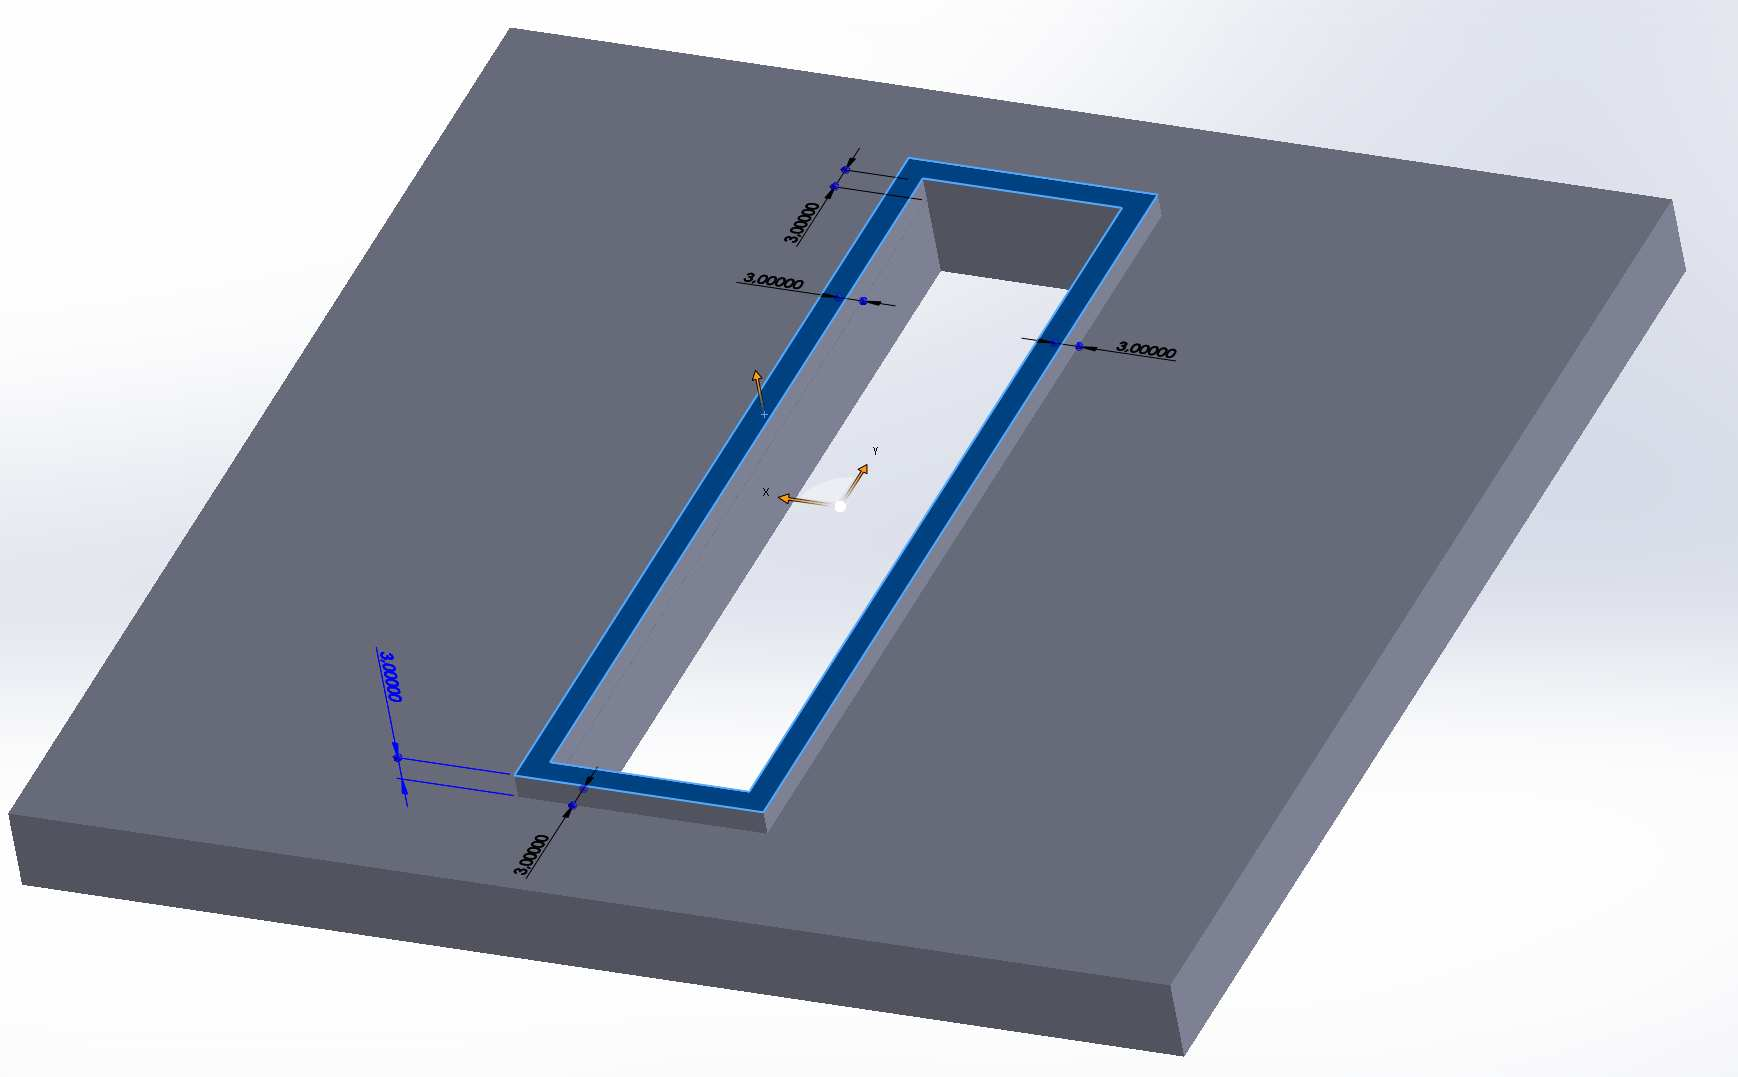
\includegraphics[width= 0.4\textwidth ]{./images/ExampleCavity.jpg}
%	\caption{Example Cavity for F20\_B and G horizontal including $3\si{\milli\meter}$ boarder. }
%	\label{fig:exampleCavity}
%\end{figure}




\begin{figure}[h!]
	\centering

	\subfloat[The PPT platform including five cavity tile.]{%
	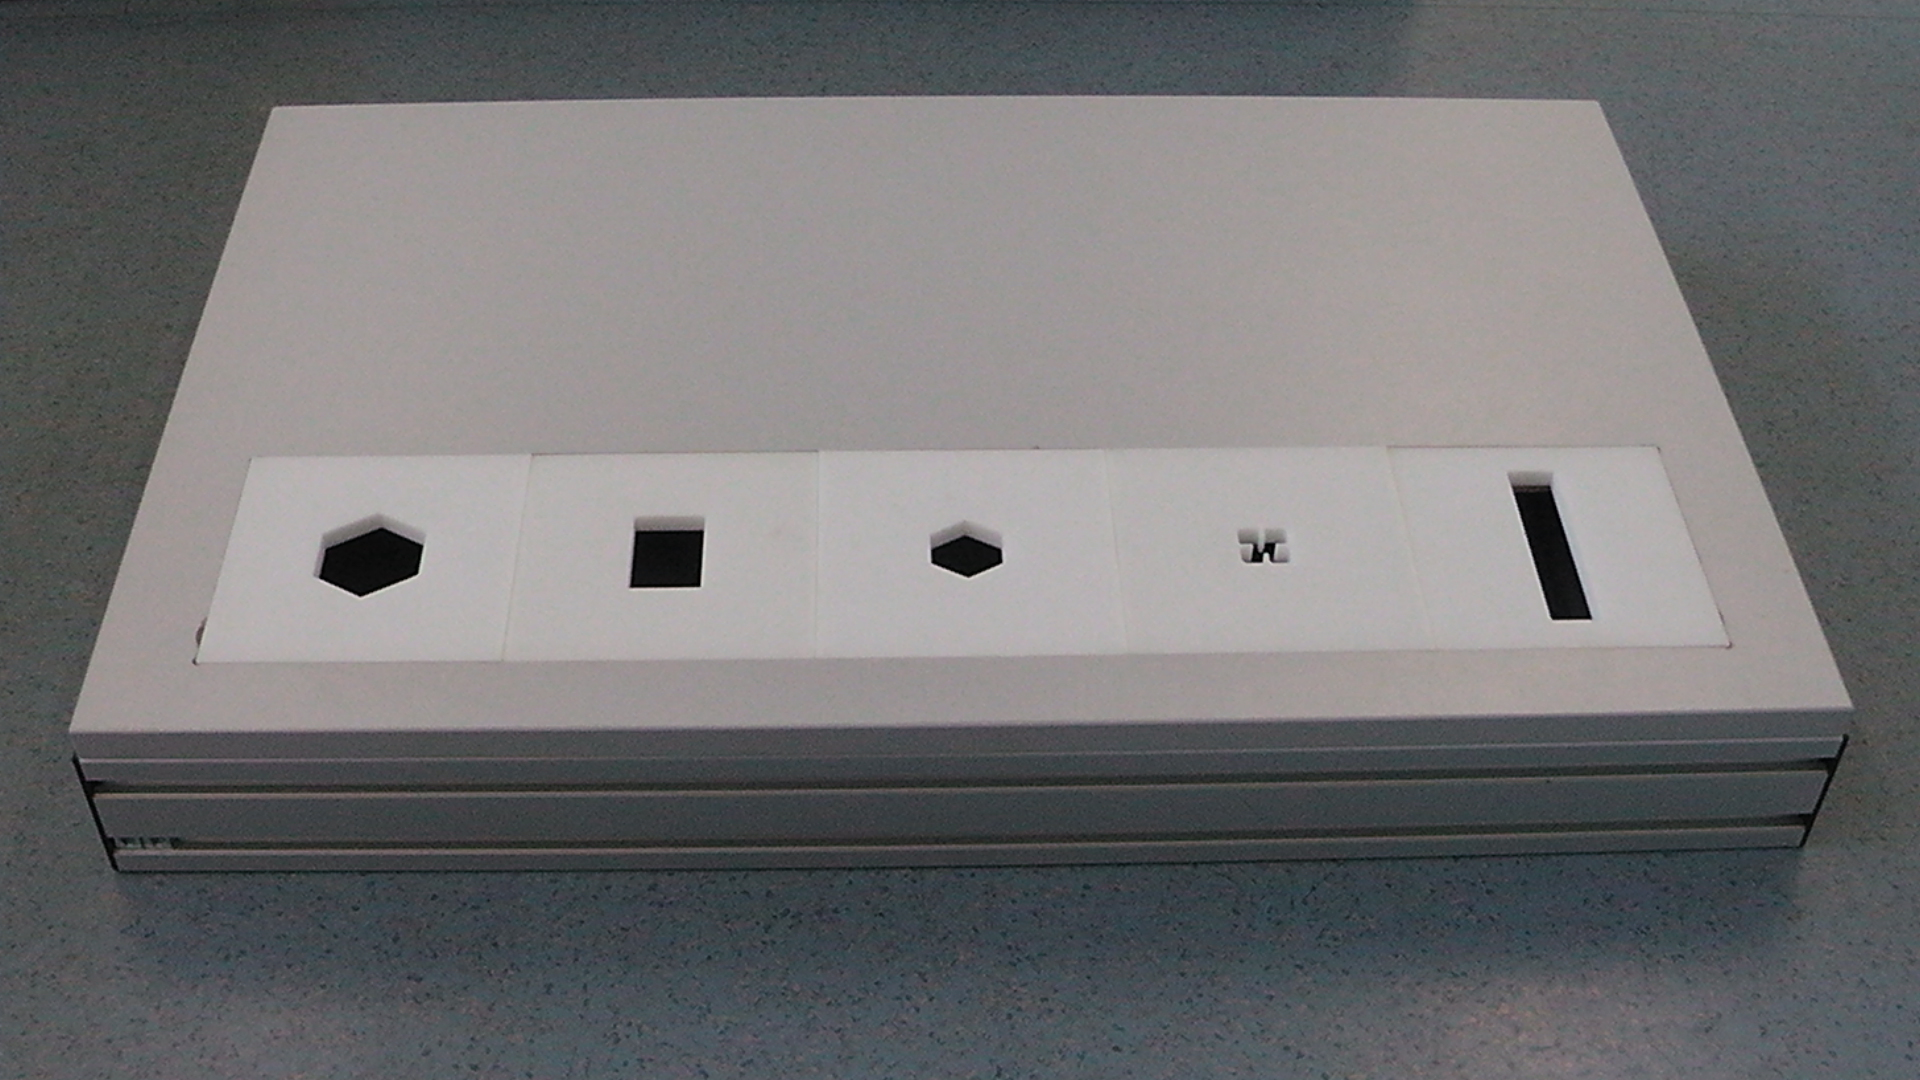
\includegraphics[width=0.45\textwidth ]{./images/ppt_plattform.jpg}
	}%
	\hspace{0.05\textwidth}
	\subfloat[Technical draw of Precision Placement table.]{%
		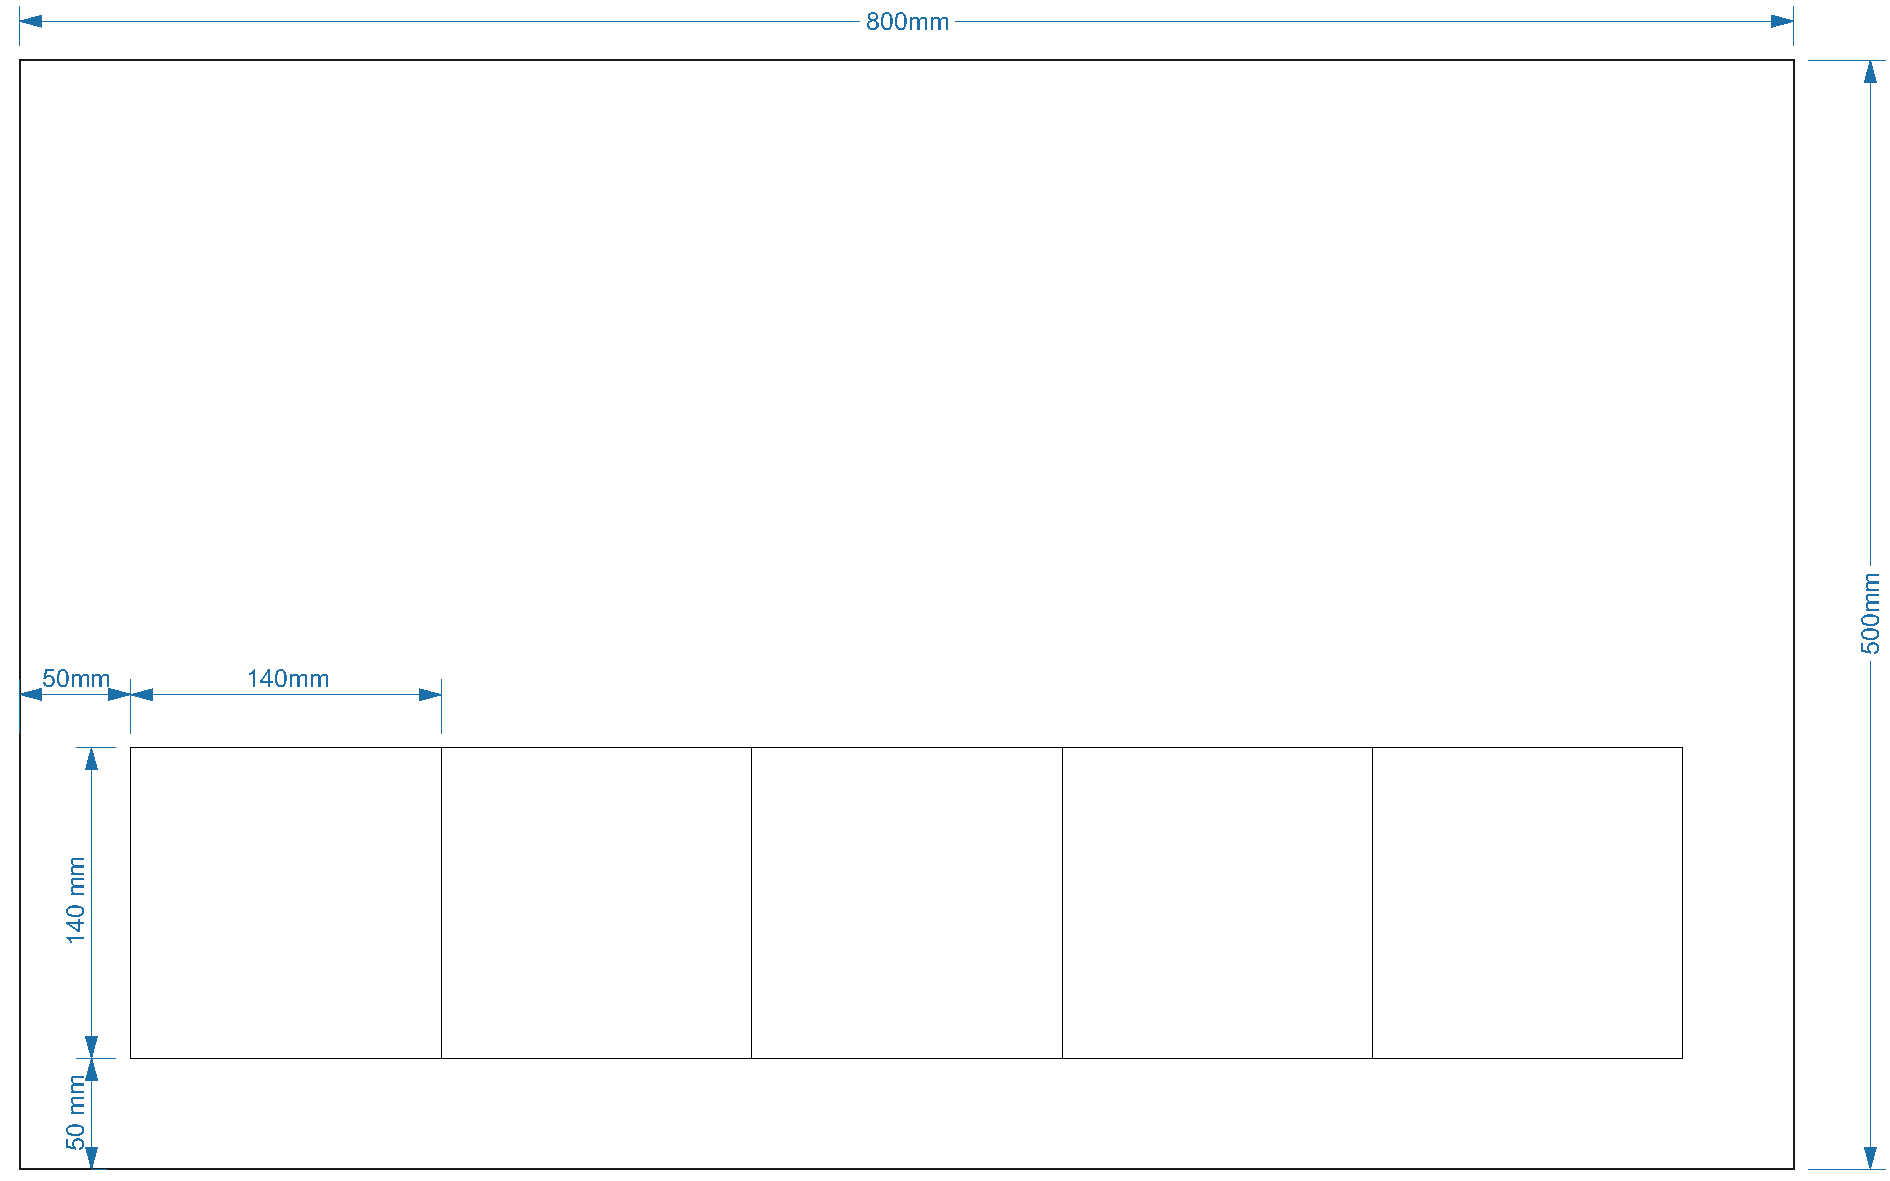
\includegraphics[width=0.45\textwidth ]{./images/PPTtable.pdf}
	}
	\caption{Exemplary Precision Placement table and generic technical drawing.}%
	\label{fig:ppt_table}
\end{figure}

\clearpage

\section{Service Areas}
\label{sec:Service_Areas}
A Service Area indicates a location for a robot where tasks (e.g. picking or placing Objects) have to be performed.
\subsection{General} 
\label{subsec:Service_Areas_General}


Such a location is usually a Table with a flat white top (see fig. \ref{fig:arena_example}), commonly referred to as Workstation (only in a case of a normal Table), but can also be a Rotating Table, Shelf, Precise Placement station or any other type needed for a specific task.
In order to successfully reach a Service Area, robots must position themselves in front of the Service Area in a way that allows manipulation of the Objects of interest and the robot has to stand still. To enable robots to reach such a position, a rectangular area with $80\si{\centi\meter}$ width must be kept free of Obstacles (see fig. \ref{fig:arena_service_area_free}). 

\begin{figure} [h!]
	\centering
	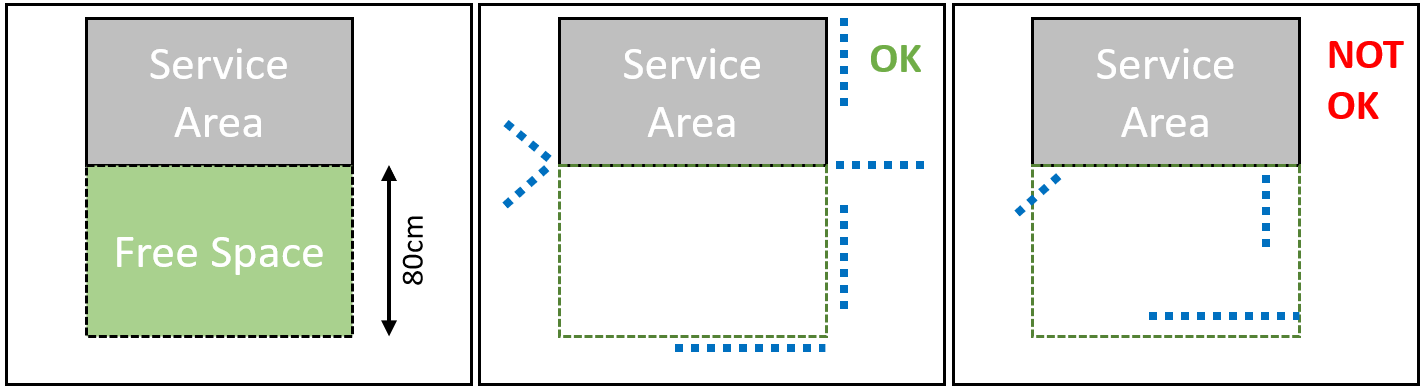
\includegraphics[width= 0.8\textwidth ]{./images/general_rules/arena_service_area_free_space}
	\caption{Free Space in front of a Service Area}
	\label{fig:arena_service_area_free}
\end{figure}

The arena layout must define where the "front" of a table is.
Figure \ref{fig:arena_map_annotated} gives an example for the definition of the position of each Service Area, marking them as WSx (Workstation x), SHx (Shelf x), PPx (Precise Placement x)and RTx (Rotating Table x). The orientation only indicates the direction of the Service Area. It does not specify the robot's heading, which may be chosen by teams according to their individual robot design.

Tables that includes Service Areas which can be used from both sides (see fig. \ref{fig:arena_example}) are defined as two seperate workstations (e.g. WS5 \& WS6). However, manipulation of theses Service Area requires the robot to have its center in the rectangular area defined in fig.~\ref{fig:arena_service_area_free}. This means that manipulation of the opposite Service Area is NOT allowed (see \ref{ssec:ManipulationZone}), even though it would be physically possible.

This rule also applies to the two positions for the Rotating table (RT1 and RT2).
This makes smaller physical layouts possible that still provide the ability to create complex navigation challenges due to the amount of locations to visit.


\subsection{Arbitrary Surfaces and Decoys}
\label{subsec:Arbitrary_Surfaces_and_Decoys}

In order to make the operating environment more realistic, the Service Areas may contain different kinds of Arbitrary Surfaces (Figure \ref{fig:ast_surface_example}) with industrial items as Decoys (Figure \ref{fig:ast_example}). The Arbitrary Surfaces don't have to be fixed mounted at the Service Areas. Examples of Arbitrary Surfaces can be different wood pattern, grass, alufoil, plexiglas etc. The integration of Arbitrary Surfaces and Decoys into tests is according the table \ref{tab:Instances}.


\begin{figure}[h!]
	\centering
	\subfloat[]{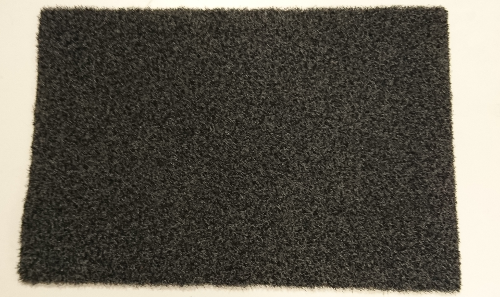
\includegraphics[width=.23333\textwidth]{./images/Arbitrary_Surface_rug}}
	\hspace{.05\textwidth}
	\subfloat[]{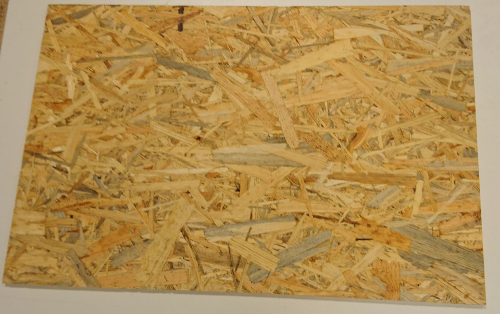
\includegraphics[width=.23333\textwidth]{./images/Arbitrary_Surface_wood}}
	\hspace{.05\textwidth}
	\subfloat[]{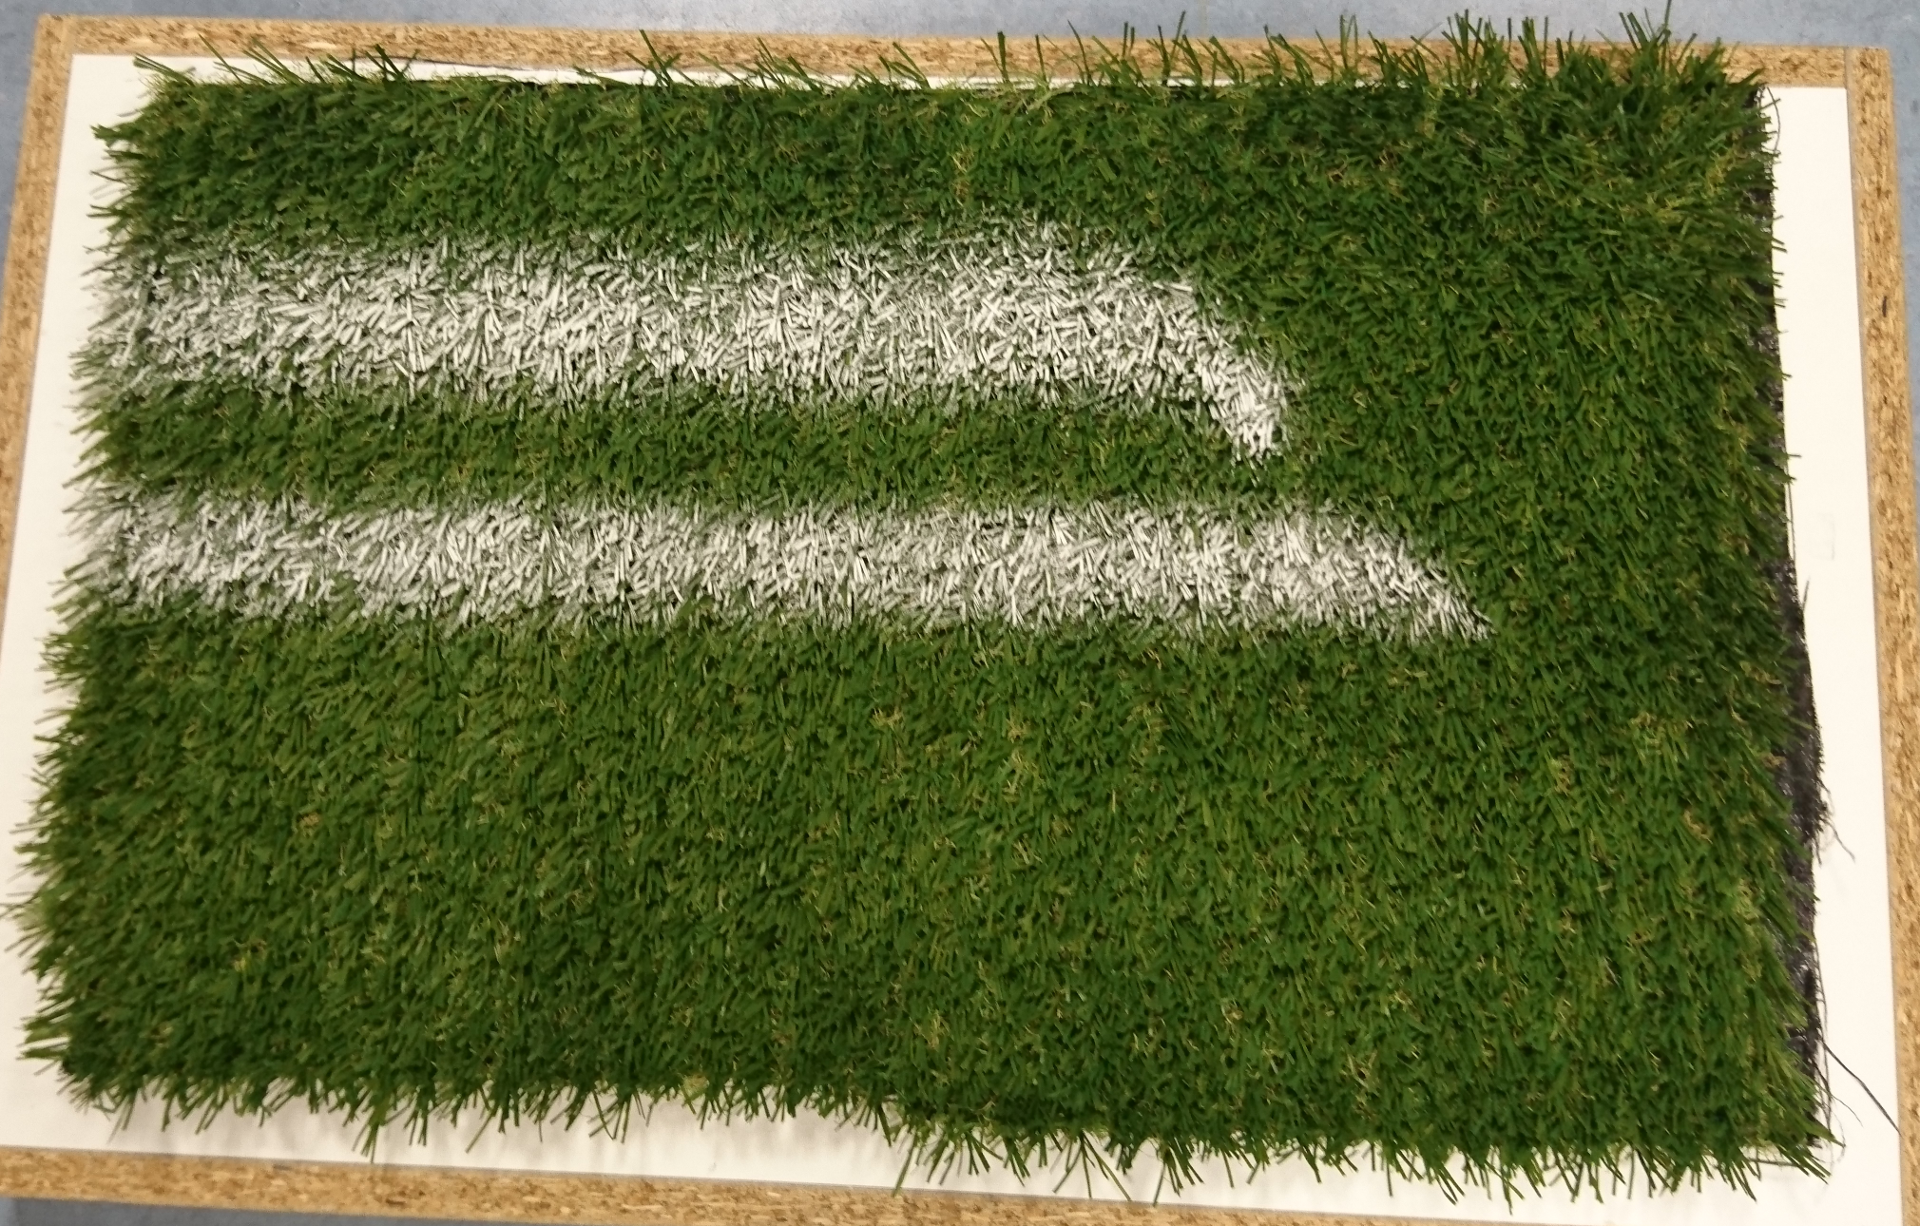
\includegraphics[width=.23333\textwidth]{./images/Arbitrary_Surface_grass}}\\
	\subfloat[]{\includegraphics[width=.23333\textwidth]{./images/Arbitrary_Surface_fake_wood_1}}
	\hspace{.05\textwidth}
	\subfloat[]{\includegraphics[width=.263333\textwidth]{./images/Arbitrary_Surface_fake_wood_2}}
	\caption{Examples of arbitrary surfaces used for Service Areas.}
	\label{fig:ast_surface_example}
\end{figure}

\begin{figure}[h!]
	\begin{center}
		\subfloat[]{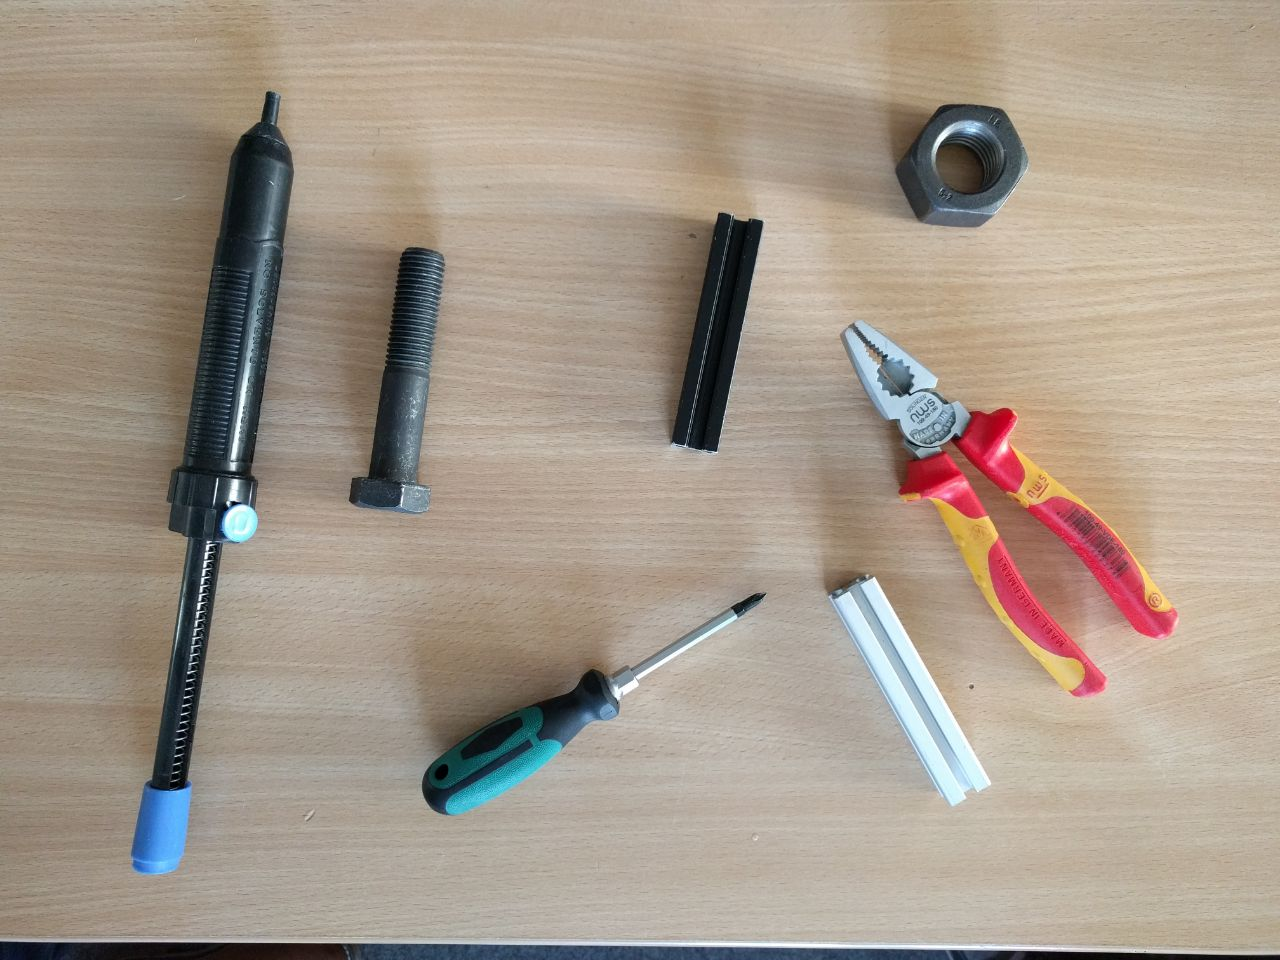
\includegraphics[width=.375\textwidth]{./images/realisticWorkingDeskI.jpeg}}
		\hspace{.05\textwidth}
		\subfloat[]{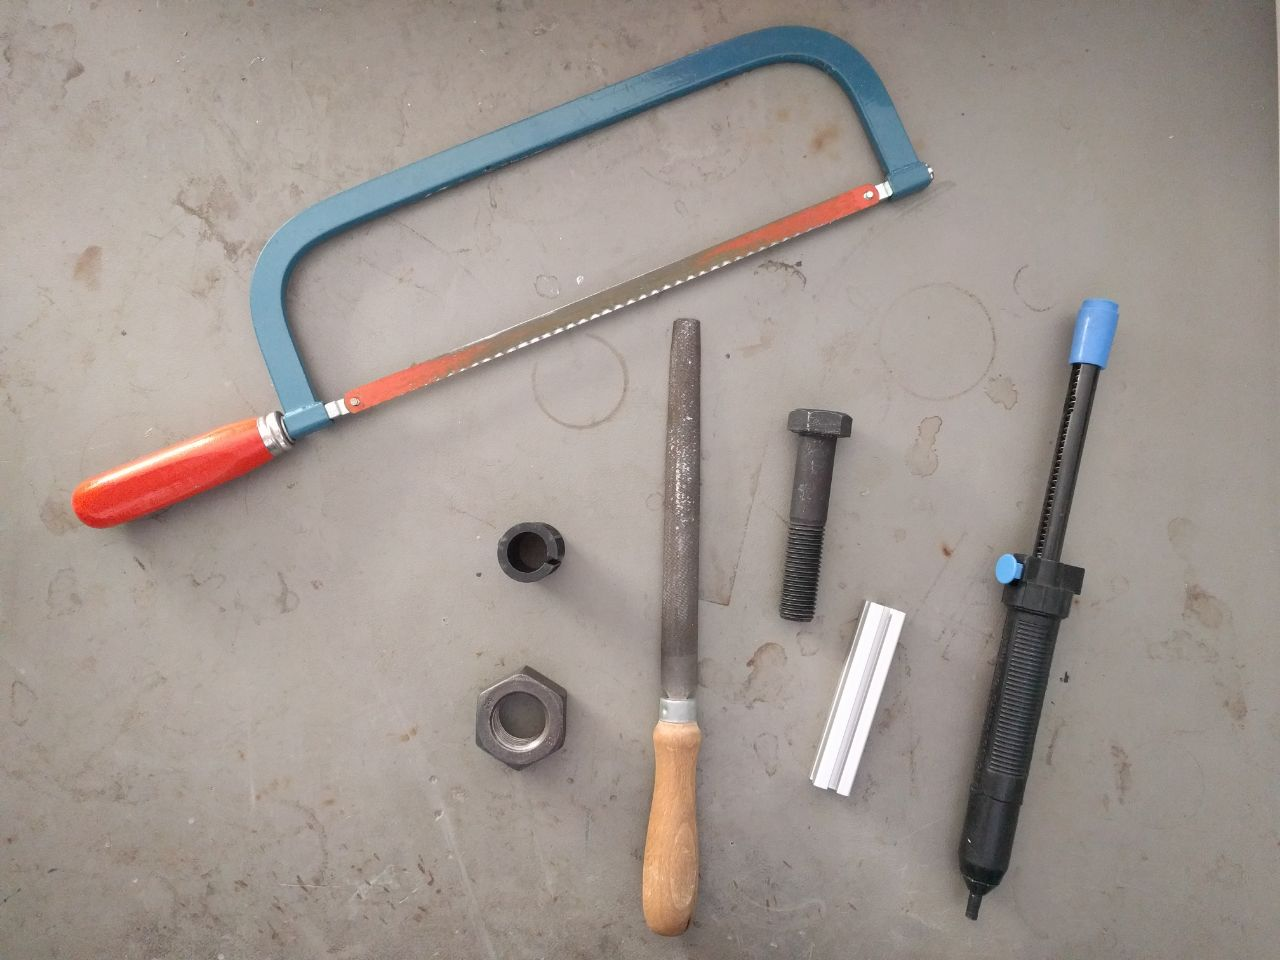
\includegraphics[width=.375\textwidth]{./images/realisticWorkingDeskII.jpeg}}
	\end{center}
	\caption{Examplary configuration of the working desks including objects and decoys.}
	\label{fig:ast_example}
\end{figure}

Placement of Decoys and arbitrary surfaces are done by the referees. Decoys could be any kind of object (tools, hardware, small electrical devices) but also standard objects from the rule book defined in section~\ref{ssec:ManipulationObjects} can be used. Figure~\ref{fig:ast_example} shows some examples. 



\subsection{Containers}
As in many industrial settings, the \RCAW environment may be equipped with several Containers (see Figure~\ref{fig:containers}). The Containers are defined as industrial plastic stacking boxes size 2B, outer dimensions: $135 \times 160 \times 82  \si{\milli\meter}$, usable dimensions: $120 \times 125 \times 65  \si{\milli\meter}$  in red ca. RAL 3020 and blue ca. RAL 5015.
% \href{https://www.amazon.de/gp/product/B0062TUUOE/ref=ppx_yo_dt_b_asin_title_o01_s00?ie=UTF8&psc=1}{example Container from amazon} (visited Januar 2022). 
They can store any kind of Object defined in Section~\ref{ssec:ManipulationObjects}. Robots are supposed either to grasp one or multiple Objects out of Containers or to place previously grasped Objects into them. Several Containers can be present in the environment and are always associated with a Service Area. That means that the Container itself will be placed within the manipulation zone defined in Section~\ref{ssec:ManipulationZone}.
It is also possible that more than one Container is placed at a single Service Area, but not multiple Containers of the same color.
The constraints defined in Section~\ref{ssec:ManipulationZone} apply also to the Containers.
Currently, a Container itself does not need to be manipulated or transported by the robot. The position of the Containers will be decided by the referees before every run type.

\begin{figure} [h!]
	\begin{center}
		\subfloat[blue]{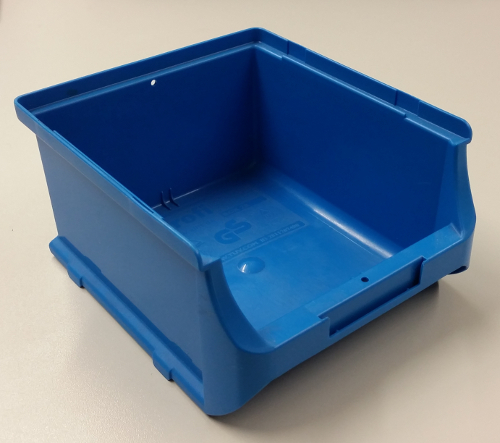
\includegraphics[width= 0.375\textwidth]{./images/container_blue.jpg}} 
		\hspace{0.05\textwidth}
		\subfloat[red]{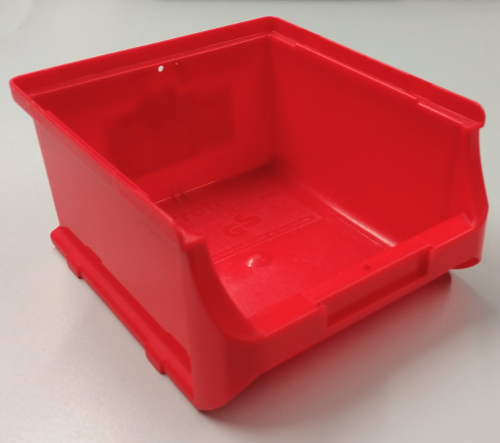
\includegraphics[width= 0.375\textwidth]{./images/container_red.jpg}}
	\end{center}
	\caption{Containers can be used for grasping Objects out or placing Objects into them.}
	\label{fig:containers}
\end{figure}


\subsection{Manipulation Zone} \label{ssec:ManipulationZone}
The manipulation zone defines the area where Objects can be placed. Thereby, the following constraints need to be satisfied:
\begin{itemize}
	\item The maximum depth of the manipulation zone is $20\si{\centi\meter}$.
	\item The minimum distance between Objects to each other is $2\si{\centi\meter}$.
	\item The minimum distance of the beginning of the manipulation zone to a Wall is $10\si{\centi\meter}$.
	\item There as an offset of $2\si{\centi\meter}$ from the border of the Service Area to the manipulation zone.
\end{itemize}
Note, the constraints do not permit, that Objects can be partially occluded dependent on the viewpoint.

For the placement of Objects the following terms are used:

\begin{itemize}
	\item Position: point within 2D coordinate system of a Manipulation Zone,
	\item Rotation: rotation around vertical axis of a Manipulation Zone,
	\item Orientation: rotation around horizontal axes of a Manipulation Zone, i.e. whether the Object is standing upright or lying on its side
	\item Pose: combination of position, rotation and orientation.
\end{itemize}
\begin{figure} [h!]
\centering
\includegraphics[width=0.8\textwidth ]{./images/manipulation_zone2023.pdf}
\caption{Manipulation zone: the green color indicates the area where Objects can be placed on a Service Area by the referees.}
\label{fig:manipulation_zone}
\end{figure}

\clearpage
\section{Objects} 
\label{ssec:ManipulationObjects}

The Objects in \RCAW include a wide range of Objects relevant in industrial applications of robotics. They eventually cover any raw material, (semi-)finished parts or products as well as tools and possibly operating materials required for manufacturing processes. \textcolor{red}{Object types are selected by the TC and shall vary in complexity due to different shapes, colors and uses of objects.}

\textcolor{red}{The basic set of Objects (called @work Object Set) includes standard profile rails, screws and nuts with various sizes and masses (see table~\ref{tab:manipulation_objects}).}

%TODO: Still need this or can we remove it with introduction of new object set?
%
%Additionally, a set of so called RoCKIn objects is used in the competition (see table~\ref{tab:manipulation_objects_rockin}). 
%These parts build a drive train of a KUKA youbot and might be used for assembly tasks.
%\textbf{REMARK:} Due to poor availability of the original RoCKin object set, teams are allowed to to use a set of 3D printed copies. The material used for fabrication has to be in standard grey/silver colour using fine quality settings and PLA as printing material. 
%An example is given with PLA Silver (ca. RAL 9006), thickness 1.75 or 2.85, not specified in detail.

%\href{https://www.amazon.de/-/en/TINMORRY-1-75mm-Filament-Printer-Spool/dp/B089YX78N5/ref=sr_1_6?crid=ZTL2O0EL3B3B&keywords=pla%2Bfilament%2Bgrau%2Bral%2B9006&qid=1641982915&s=industrial&sprefix=pla%2Bfilament%2Bgrau%2Bral9006%2Cindustrial%2C114&sr=1-6&th=1 }{example material from amazon} (visited Januar 2022). 
%Figure~\ref{fig:RoCKIn_printed} shows an example set of the printed RoCKIn Objects created using fused filament fabrication (FFF) printing. 

\textcolor{red}{In 2023, the RoCKIn object set (see 2022 rulebook or previous ones) is finally replaced by a selection of better available parts for a drive train, as well as some tools (see Section~
\ref{sec:new_objects}). The new object set was introduced in a technical challenge in 2022 and is called Advanced Object Set.}

\textcolor{red}{The exact appearance of the object used in the competition can slightly vary, e.g. different coating colors for some standard parts.}

% as shown in  and . Objects of one kind can slightly vary e.g. considering the surface and coating colour. 

%RoCKIn Objects are spare parts from the KUKA you-bot platform often used in the competition, due to the fact that the KUKA you-bot and the RoCKIn Objects are not longer produced in future those Objects will be replaced with other standard parts used in industry as shown in Section~
%\ref{sec:new_objects}. 




\subsection{\textcolor{red}{Basic} Object Set}


\newcommand{\imageView}[1]{\includegraphics[width=2cm, valign=c]{#1}}
{
\newcommand{\rowpadding}{0.4cm}
\setlength\extrarowheight{\rowpadding}
\begin{table}[p]

\begin{tabular}{|c|c|c|c|m{8cm}|}
\hline
ID & Object & Symbolic Description & Mass & Details \\
\hline

\texttt{1} & \imageView{./images/F20_20_B.jpg} & \texttt{F20\_20\_B} & 49 g & Small aluminium profile \newline
 Coating/Colour: black anodized\newline
 Height: 20 mm \newline
 Width: 20 mm \newline
 Length: 100 mm \\ [\rowpadding]
\hline

\texttt{2} & \imageView{./images/F20_20_G.jpg} & \texttt{F20\_20\_G} & 49 g & Small aluminium profile \newline
 Coating/Colour: gray anodized\newline
 Height: 20 mm \newline
 Width: 20 mm \newline
 Length: 100 mm \\ [\rowpadding]
\hline

\texttt{3} & \imageView{./images/S40_40_B.jpg} & \texttt{S40\_40\_B} & 186 g & Big aluminium profile\newline
 Coating/Colour: black anodized\newline
 Height: 40 mm \newline
 Width: 40 mm \newline
 Length: 100 mm \\ [\rowpadding]
\hline

\texttt{4} & \imageView{./images/S40_40_G.jpg} & \texttt{S40\_40\_G} & 186 g & Big aluminium profile \newline
 Coating/Colour:  gray anodized\newline
 Height: 40 mm \newline
 Width: 40 mm \newline
 Length: 100 mm \\ [\rowpadding]
\hline

\texttt{5} & \imageView{./images/M20_100.jpg} & \texttt{M20\_100} & 296 g & Screw\newline
 ISO4014, DIN 931, CSN 021101, PN 82101, UNI 5737, EU 24014 \newline
 Coating/Colour: blank, black burnished \newline
 Size: M$20\times 100$ \\ [\rowpadding]
\hline

\texttt{6} & \imageView{./images/M20.jpg} & \texttt{M20} & 56 g & Small nut\newline
 ISO4032, DIN934,  CSN 021401, PN 82144, UNI 5588, EU 24032  \newline
 Coating/Colour: blank, black burnished \newline
 Size: M20 \\ [\rowpadding]
\hline

\texttt{7} & \imageView{./images/M30.jpg} & \texttt{M30} & 217 g & Big nut\newline
 ISO4032, DIN934,  CSN 021401, PN 82144, UNI 5588, EU 24032  \newline
 Coating/Colour: blank, black burnished \newline
 Size: M30 \\ [\rowpadding]
 \hline
\end{tabular}
\caption{\RCAW Object set.}
\label{tab:manipulation_objects}
\end{table}



\clearpage
%\subsection{RoCKIn Object Set}
%
%\subsubsection{Original Set}
%
%
%\begin{table}[h!]
%\begin{tabular}{|c|c|c|c|m{6cm}|}
%\hline
%ID & Object & Symbolic Description & Mass & Details \\
%\hline
%
%\texttt{8} & \imageView{./images/bearingBoxA.jpg} & \texttt{Bearing\_Box} & 102 g & Bearing box\newline
% Height: 25 mm \newline
% Width: 45 mm \newline
% Length: 50 mm \newline
% Inner diameter: 32 mm \\ [\rowpadding]
%\hline
%
%\texttt{9} & \imageView{./images/bearing.jpg} & \texttt{Bearing} & 42 g & Bearing\newline
% Height: 13 mm \newline
% Inner diameter: 15 mm \newline
% Outer diameter: 32 mm \\ [\rowpadding]
%\hline
%
%\texttt{10} & \imageView{./images/axis.jpg} & \texttt{Axis} & 40 g & Axis\newline
% Diameter: 27 mm \newline
% Length: 96 mm \\ [\rowpadding]
%\hline
%
%\texttt{11} & \imageView{./images/distanceTube.jpg} & \texttt{Distance\_Tube} & 5 g & Distance tube\newline
% Height: 10 mm \newline
% Inner diameter: 28 mm \newline
% Outer diameter: 32 mm \\ [\rowpadding]
%\hline
%
%\texttt{12} & \imageView{./images/motor.jpg} & Motor & 20 g & Motor\newline
% Diameter: 42 mm \newline
% Length: 87 mm \\ [\rowpadding]
%\hline
%
%\texttt{13} & \imageView{./images/R20.jpg} & \texttt{R20} & 14 g & Plastic tube\newline
%Inner diameter: 20 mm \newline
%Outer diameter: 30 mm \newline
%Length: 45 mm \\ [\rowpadding]
%\hline
%%\imageView{./images/V20.jpg} & \texttt{V20} & 14 g & Inner diameter: 20 mm \newline
%%Outer diameter: 30 mm \newline
%%Length: 45 mm \\
%%\hline
%\end{tabular}
%\caption{RoCKIn Object set.}
%\label{tab:manipulation_objects_rockin}
%\end{table}
%}
%
%\clearpage
%\subsubsection{Printed Set}
%
%
%\begin{figure}[h!]
%	\begin{center}
%		\subfloat[]{\includegraphics[width=0.8\textwidth]{./images/rockingPrinted1.jpg}}
%		\vspace{0.05\textwidth}
%		\subfloat[]{\includegraphics[width=0.8\textwidth]{./images/rockingPrinted2.jpg}}
%	\end{center}
%	\caption{Examplary 3D printed RoCKIn Objects (bearing box, bearing, axis, distance\_tube, motor, plastic tube R20). Material:  PLA silver ( ca. RAL 9006), 2.85mm. Printer: Ultimaker 3 extended. Printer settings: fine}
%	\label{fig:RoCKIn_printed}
%\end{figure}



\clearpage
\subsection{\textcolor{red}{Advanced Object Set}}


\textcolor{red}{A new object set was introduced in 2022 as a technical challenge that is intended to introduce objects that are closer to a real-life scenario. The set includes different tools and an updated drive shaft to replace the RoCKIn set. Links for purchase can be found in \ref{sec:new_objects}.}

\begin{table}[h!]
	\begin{tabular}{|c|m{2cm}|c|c|m{8cm}|}
		\hline
		ID & Object & Symbolic Description & Mass & Details \\
		\hline
%%%%%%%%%%%%%
		\texttt{20} & \imageView{./images/newObjects/welle3d.jpg} \newline
		\imageView{./images/newObjects/welleSchematic.JPG}
		& \texttt{Axis2} & 180 g & Steel axis \newline
		Misumi: SFUB25-25-F28-P17-T15-S10-Q20 \newline
		Coating/Colour: blank, black burnished \newline
		Length: 68 mm \newline
		Diameter: 17mm, M20 \newline
		see Figure~\ref{fig:welle2Schematic} \newline
		
		\href{https://de.misumi-ec.com/vona2/detail/110302635710/?CategorySpec=00000146753%3a%3ab%2cc}{Misumi} (visited Januar 2022)\\

			\hline
%%%%%%%%%%%%
		\texttt{21} & \imageView{./images/newObjects/bearing2.JPG} & \texttt{Bearing2} & 100 g & Bearing \newline 
		SKF YAR203-2F\newline
		Coating/Colour: gray \newline
		Useable with housing\newline
		\href{https://www.skf.com/sg/products/rolling-bearings/ball-bearings/insert-bearings/productid-YAR%20203-2F}{SKF}  (visited Januar 2022)\\
		\hline
%%%%%%%%%%%%				
		\texttt{22} & \imageView{./images/newObjects/housing.JPG} & \texttt{Housing} & 60 g & Housing \newline 
		SKF P40\newline
		Coating/Colour: gray \newline
		Useable with bearing\newline
		\textbf{Remark:} needs two hex socket screw M8x10 (DIN EN ISO 4762, DIN 912, CSN 021143, PN 82302, UNI 5931) and two M8 nuts (ISO 4032, DIN 934) \newline
		\href{https://www.skf.com/sg/products/mounted-bearings/ball-bearing-units/pillow-block-ball-bearing-units/productid-P%2040}{SKF}  (visited Januar 2022)\\
		\hline
%%%%%%%%%%%%	
		\texttt{23} & \imageView{./images/newObjects/motor.JPG} & \texttt{Motor2} & 350g & Motor 755\newline
		Coating/Colour: gray \newline
		Size: $66.7 \times 42.0 \si{\milli\meter}$\newline
		Diameter: $d_{axis}=5\si{\milli\meter}$, $l_{axis}=10\si{\milli\meter}$ \newline
		\href{https://www.amazon.de/EsportsMJJ-12V-36V-3500-9000Rpm-Drehmoment-Hochleistungsmotor/dp/B075D85KVV}{Amazon}  (visited Januar 2022)\\
		\hline
%%%%%%%%%%%%					
		\texttt{24} & \imageView{./images/newObjects/FlangedResinCollar.JPG} & \texttt{Spacer} &  & Flanged Spacer\newline
		Misumi CLJHJ25-30-70  \newline
		Coating/Colour: white \newline
		Size: $70\si{\milli\meter}$\newline
		Diameter: $d_{inner}=25\si{\milli\meter}$, $d_{outer}=30\si{\milli\meter}$ \newline
		\href{https://us.misumi-ec.com/vona2/detail/110300236450/?curSearch=%7b%22field%22%3a%22%40search%22%2c%22seriesCode%22%3a%22110300236450%22%2c%22innerCode%22%3a%22%22%2c%22sort%22%3a1%2c%22specSortFlag%22%3a0%2c%22allSpecFlag%22%3a0%2c%22page%22%3a1%2c%22pageSize%22%3a%2260%22%2c%2200000042362%22%3a%22mig00000001500952%22%2c%2200000042368%22%3a%22b%22%2c%22jp000157843%22%3a%22mig00000000344081%22%2c%22jp000157846%22%3a%22mig00000001417174%22%2c%22jp000157851%22%3a%22mig00000000344088%22%2c%2200000334029%22%3a%2230%22%2c%2200000334032%22%3a%2270%22%2c%22typeCode%22%3a%22CLJHJ%22%2c%22fixedInfo%22%3a%22MDM0000085422111030023645020110476153310093415426696895%7c14%22%7d&Tab=preview}{Misumi}  (visited Januar 2022)\\
						\hline

\end{tabular}
\caption{\textcolor{red}{Advanced Object Set}}
\label{tab:new_objects1}
\end{table}


\begin{table}[h!]
	\begin{tabular}{|c|m{2cm}|c|c|m{8cm}|}
		\hline
		Object & Symbolic Description & Mass & Details \\
		\hline
		%%%%%%%%%%%%
		\texttt{24} & \imageView{./images/newObjects/weraScrewdriver.jpg} & \texttt{Screwdriver } & 19g & WERA 352 \newline
		Ball end screwdriver,hexagon socket screws\newline
		Coating/Colour: black/green \newline
		Size: $181\si{\milli\meter}$\newline
		Diameter: $d_{tip}=2.5\si{\milli\meter}$\newline
		Code: 05138070001\newline
		\href{https://www.amazon.de/Wera-05138070001-352-Sechskant-Kugelkopf-Schraubendreher-2-5/dp/B00154ZWFI?th=1}{Amazon}  (visited Januar 2022)\\
		\hline
		%%%%%%%%%%%%			
		\texttt{25} & \imageView{./images/newObjects/weraWrench.jpg} & \texttt{Wrench } & ca. 72g & WERA Jocker 6000, 8mm \newline
		Ratcheting combination wrenches\newline
		Coating/Colour: silver/grey/pink \newline
		Size: ca. $144\si{\milli\meter}$\newline
		Diameter: $d_{max}=20\si{\milli\meter}$\newline
		Code: 05073268001\newline
		\href{https://www.amazon.de/Wera-05073268001-Joker-Maul-Ringratschen-Schl%C3%BCssel/dp/B00BT0GBMG?th=1}{Amazon} (visited Januar 2022)\\
		\hline
		%%%%%%%%%%%%
		\texttt{26} & \imageView{./images/newObjects/hsscoDIN338metaldrill.jpg} & \texttt{Drill } & ca. 10g & Bosch Drill HSS-Co DIN338  \newline
		Drill\newline
		Coating/Colour: gold/ Cobalt alloy \newline
		Length: ca. $151\si{\milli\meter}$\newline
		Diameter: $d_{max}=13\si{\milli\meter}$\newline
		Code: 3165140382724 \newline
		\href{https://www.amazon.com/Bosch-2609255086-Metal-Drill-HSS-Co/dp/B0071OSFQY}{Amazon} (visited Januar 2022)\\
		\hline
		%%%%%%%%%%%
		\texttt{27} & \imageView{./images/newObjects/weraAllenKey.jpg} & \texttt{AllenKey } & ca. 10g & Wera Allen Key 8mm,\newline
		3950 PKL L-key, metric, stainless\newline
		Coating/Colour: silver \newline
		Length: ca. $195\si{\milli\meter} \times 37\si{\milli\meter}$\newline
		Diameter: $d_{max}=8\si{\milli\meter}$\newline
		Code: 05022708001 \newline
		\href{https://www.amazon.co.uk/Wera-WER022708-Hexagon-Keys-Multi-Colour/dp/B00A8QXTNG}{Amazon} (visited Januar 2022)\\
		\hline
		%%%%%%%%%%%
	
\end{tabular}
\caption{\RCAW New set of manipulation objects (tool set).}
\label{tab:new_objects2}
\end{table}

\clearpage
\subsection{April Tagged Object Set}
\label{ssec: April Tagged Object Set}

For the season 2023 and onwards, 3D printed cubes marked with April tags might be used in the competition. Further on this cubes will be called April Tag Tagged Cubes (ATTC).
This shall prepare the possibility to design tasks that focus on other areas than object recognition by simplifying the detection. 
All April Tags will be $40 \si{\milli\meter} \times 40 \si{\milli\meter}$ and out of the \textit{36h11} April Tag Family, including 1bit black, 1bit white boarder as shown in fig. \ref{fig:singleAprilTag}. 

\begin{figure}[h!]
	\centering
	\includegraphics[width= 0.4\textwidth ]{./images/singleAprilTAG42.png}
	\caption{Example of an April Tag with the ID: 42 out of the 36h11-April Tag Family.}
	\label{fig:singleAprilTag}
\end{figure}

All the used April Tag ID numbers will fit to the ID numbers used by the AtWork Commander. 
%
%uint16 EMPTY = 0
%
%# atwork
%uint16 ATWORK_START = 11
%uint16 F20_20_B = 11
%uint16 F20_20_G = 12
%uint16 S40_40_B = 13
%uint16 S40_40_G = 14
%uint16 M20_100 = 15
%uint16 M20 = 16
%uint16 M30 = 17
%uint16 R20 = 18
%uint16 ATWORK_END = 19
%
%# rockin
%uint16 ROCKIN_START = 21
%uint16 BEARING_BOX = 21
%uint16 BEARING = 22
%uint16 AXIS = 23
%uint16 DISTANCE_TUBE = 24
%uint16 MOTOR = 25
%uint16 ROCKIN_END = 26
%
%# container
%uint16 CONTAINER_START = 31
%uint16 CONTAINER_RED = 31
%uint16 CONTAINER_BLUE = 32
%uint16 CONTAINER_END = 33
%
%# cavity
%uint16 CAVITY_START = 41
%uint16 F20_20_H  = 41
%uint16 F20_20_V  = 42
%uint16 F20_20_F  = 43
%uint16 S40_40_H  = 44
%uint16 S40_40_V  = 45
%uint16 S40_40_F  = 46
%uint16 M20_H     = 47
%uint16 M20_V     = 48
%uint16 M20_F     = 49
%uint16 M20_100_H = 50
%uint16 M20_100_V = 51
%uint16 M20_100_F = 52
%uint16 M30_H     = 53
%uint16 M30_V     = 54
%uint16 M30_F     = 55
%uint16 R20_H     = 56
%uint16 R20_V     = 57
%uint16 R20_F     = 58
%uint16 CAVITY_END = 59 




\subsubsection{ATTC as Manipulation Objects}

The standard ATTC measures $42\si{\milli\meter} \times 42\si{\milli\meter} \times 42 \si{\milli\meter}$ and has slightly rounded edges, similar to the shape of aluminum profile rails. On the top there is a $1\si{\milli\meter}$ deep cavatie ( $40.5\si{\milli\meter} \times 40.5\si{\milli\meter}$) to place the individual April Tag. It is manufactured by 3D printing using PLA filament of any color. The april tag is glued to the top side of the ATTC and is encoded with an ID matching one of the objects.
The exact design and size is specified in fig. \ref{fig:cubeObject} and can be downloaded from the official league repository: \href{https://github.com/robocup-at-work/rulebook/tree/alpha_2023/images}{3D STL file of manipulation Cube.}
The sides are marked with the ID in numeric numbers to make the cubes also identifyable by humans.

\begin{figure}[h!]
	\centering
	\subfloat[April Tag Tagged Cube (ATTC), including overall dimensions.]{\includegraphics[width=0.375\textwidth ]{./images/AprilTags/AprilTagCube2023_2.png}}
	\hspace{0.05\textwidth}
	\subfloat[Detailed dimensions of the ATTC cavaty to fix a certain April Tag.]{ \includegraphics[width=0.375\textwidth ]{./images/AprilTags/AprilTagCube2023_1.png} }
	\caption{3D construction of the ATTC as manipulation object.}%
	\label{fig:cubeObject}
\end{figure}

\subsubsection{Tagged Targets}

Target objects, such as a precise placement cavity or a container, might also be marked with an April Tag.

For the PP cavaty tiles, one design will be used for all ATTC with any object ID. The design foresees a matching hole and two square cut-outs where tagged plates can be inserted. Additional to the April Tag also the April Tag ID will be shown on the tile.
The ID used matches the ID used in the Atwork Commander so it should also mach with the correct ATTC.
See the schematics shown in fig. \ref{fig:cubeObjectTile} for details. 

\begin{figure}[h!]
	\centering
	\subfloat[ATTC cavity tile, including overall dimensions.]{\includegraphics[width=0.375\textwidth ]{./images/AprilTags/CubeTile2023_2.png}}
	\hspace{0.05\textwidth}
	\subfloat[Detailed dimensions of the ATTC tile April Tag cavatie.]{ \includegraphics[width=0.375\textwidth ]{./images/AprilTags/CubeTile2023_1.png} }
	\caption{3D construction  of the ATTC Precision Placement cavaty tile.}%
	\label{fig:cubeObjectTile}
\end{figure}

Containers get an April tag glued onto the inside of the bottom surface with centric placement as shown in fig. \ref{fig:redContainerTagged}.

\begin{figure}[h!]
	\centering
	\includegraphics[width= 0.5\textwidth ]{./images/AprilTags/container_redTAG.png}
	\caption{Example of a red container, tagged with the April Tag ID: "31".}
	\label{fig:redContainerTagged}
\end{figure}


\subsubsection{April Tags}
April Tags can be easy generated. The usage of any ROS package to identify the April Tag is allowed. For example the \href{http://wiki.ros.org/apriltag_ros}{April Tag ROS package} can easy be adapted to be used within the competition. Example April Tags out of the April Tag Family  36h11 are shown in fig. \ref{fig:AprilTagExamples}. 


\begin{figure}[h!]
	\centering
	\includegraphics[width= 0.8\textwidth ]{./images/AprilTags/AprilTags0TO31.png}
	\caption{Examples of April Tags with $0 \le April Tag ID \le 31$.}
	\label{fig:AprilTagExamples}
\end{figure}










